\documentclass[11pt]{beamer} % mathserif for normal math fonts.
\usefonttheme[onlymath]{serif}
\usepackage[utf8]{inputenc}
\usepackage[swedish,english]{babel}
\usepackage{microtype}
\usepackage{calc}
\usepackage{amsmath,mathtools}
\usepackage[backend=biber]{biblatex}
\usepackage{contmech}
%\usepackage{subfig}
%\usepackage{siunitx}
%\usepackage{movie15}
\usepackage{wasysym}
\usepackage{multimedia}
\usepackage{grffile}
\usepackage{tikz}
\usepackage{pgfplots}

%\pgfplotsset{compat=newest}
\pgfplotsset{compat=1.6}
\usetikzlibrary{shapes,arrows}

\newcommand{\highlight}[1]{{\color{red}#1}}
\newcommand{\downlight}[1]{{\color{gray}#1}}
\DeclarePairedDelimiter{\homgen}{\langle}{\rangle_\rve}
\DeclarePairedDelimiter{\shomgen}{\langle\!\langle}{\rangle\!\rangle_\rve}
\DeclarePairedDelimiter{\jmp}{[\![}{]\!]}
\newcommand{\jump}[1]{[\![#1]\!]}
\newcommand{\prescribed}{\mathrm{pre}}
\newcommand{\on}{\quad\text{ on }}
\renewcommand{\dev}{\mathrm{d}}
\renewcommand{\vol}{\mathrm{v}}
\newcommand{\per}{\mathrm{per}}
\newcommand{\volume}{|\Omega_\rve|}
\newcommand{\ded}{\mathrm{d}}
\newcommand{\dep}{\mathrm{p}}
\newcommand{\Periodic}{\mathrm{P}}
\newcommand{\external}{\mathrm{ext}}
\newcommand{\surf}{\mathrm{s}}
\newcommand{\pore}{\mathrm{pore}}
\newcommand{\particle}{\mathrm{part}}
\newcommand{\devop}{\ts\epsilon_\dev}
\newcommand{\densinv}{\eta}
\newcommand{\dens}{\eta^{-1}}
\newcommand{\epspargs}{\{{\bar{\ts d}}_\dev, \bar{p}\}}
\newcommand{\rve}{
  {\mathchoice
   {\mbox{\scalebox{0.67}{$\Box$}}}
   {\mbox{\scalebox{0.67}{$\Box$}}}
   {\mbox{\scalebox{0.5}{$\Box$}}}
   {\mbox{\scalebox{0.375}{$\Box$}}}
  }
}
%\usepgfplotslibrary{patchplots}
%\usepgfplotslibrary{groupplots}
%\pgfplotsset{compat=1.3}

\newcommand{\roughcite}[1]{\textsc{#1}}
\renewcommand{\alert}[1]{\textbf{#1}}

\setbeamersize{text margin left=.3cm,text margin right=.3cm}

\usetheme[titleflower=true]{chalmers}
\title{
On computational modeling of sintering based on homogenization
}
\author[Mikael \"Ohman Ph.D.\ defence  --- 2014-06-13]{Mikael \"Ohman}
\institute{Department of Applied Mechanics\\ Chalmers University of Technology\\
mikael.ohman@chalmers.se
}
%\titlepageextra{2012}% session: Multiple-scale physics and computation
\date{2014-06-13}
%\footer{\insertshortauthor\ 2\textsuperscript{nd} ICMM}
\titlepagelogofile{Avancez_gold}

% Bibliography
%\bibliography{references_extended}

% Speeds up compilation.
% \usetikzlibrary{external}
% \tikzexternalize


\addbibresource{Multiscale.bib} % New command, use if available
\addbibresource{Sintering.bib}

\begin{document}

\section{Title page}
\begin{frame}[plain]
 \titlepage
\end{frame}

\section{Acknowledgement}
\begin{frame}
 \frametitle{Acknowledgement}
 \begin{center}
 Funding:
 \\
 Swedish Research Council (Vetenskapsrådet)
 \\
 Chalmers University of Technology
 \\[2em]
 Supervisors:\\
 Professor Kenneth Runesson \\
 Professor Fredrik Larsson
 \end{center}
\end{frame}

\section{Outline}
\begin{frame}
 \frametitle{Outline}

\begin{itemize}
 \item Motivation of project / background on sintering
 \item Classical (macroscale) constitutive modeling of sintering
 \item Fine scale problem
 \item Two-scale problem -- Paper A--D
%  \begin{itemize}
%   \item Paper A --- Computational mesoscale modeling and homogenization of liquid-phase sintering of particle agglomerates
%   \item Paper B --- Computational homogenization of liquid-phase sintering with seamless transition from macroscopic compressibility to incompressibility
%   \item Paper C --- On the variationally consistent computational homogenization of elasticity in the incompressible limit
%   \item Paper D --- A mixed variational format for two-scale analysis of liquid-phase sintering based on variationally consistent homogenization
%  \end{itemize}
 \item Conclusions
 \item Future work
\end{itemize}
\end{frame}

%%%%%%%%%%%%%%%%%%%%%%%%%%%%%%%%%%%%%%%%%%%%%%%%%%%%%%%%%%%%%%%%%%%%%%%%%%%%%%%%%%%%%%%%%%%%%%%%%%%
\section{Background}
\begin{frame}
 \frametitle{Motivation --- Sintering of hardmetal}

% The sintering phenomenon on the mesoscale is driven by surface tension on the melted binder, and
% the homogenized effect of the surface tension is the so-called sintering stress.
% From the macroscopic perspective, the specimen (green body) shrinks due to this volumetric sintering stress. In the case of inhomogeneous
% initial density in the green body, the sintering can result in unwanted final deformations.

 \begin{enumerate}
  \item WC-particles in Co-matrix (binder metal)
  \item Precompaction $\rightarrow$ inhomogeneous ``green body'', porosity $\phi_0\approx$ 0.2--0.4
  \item Heating $\rightarrow$ thermal expansion, sintering driven by surface tension in melted Co, i.e. ``liquid phase sintering'' $\rightarrow$
        Fully dense final product $\phi=0$.
 \end{enumerate}
\alert{Note:} Inhomogeneous initial density may lead to defect product:\\ \textsuperscript{(i)}remaining porosity, \textsuperscript{(ii)}shape imperfection\\
\alert{Note:} Macroscopic compressibility despite \underline{assumed} intrinsic incompressibility of constituents until $\phi = 0$.
\begin{center}
 \begin{columns}
 \column{0.25\textwidth}\centering
 \begin{tikzpicture}
   \node at (0,0) {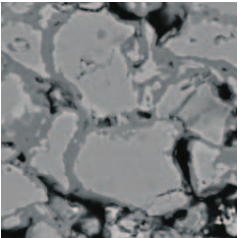
\includegraphics[width=\textwidth]{figures/sinter_1-crop.pdf}};
   \draw[red,thick,<-] (1,1) -- (1.5,1) node[right,black] {WC};
   \draw[red,thick,<-] (0.5,0.7) -- (1.5,0.5) node[right,black] {Co};
   \draw[red,thick,<-] (0.7,-0.3) -- (1.5,0) node[right,black] {pore};
 \end{tikzpicture}
 \column{0.05\textwidth}\centering
 $\xrightarrow{\text{idealized}}$
 \column{0.25\textwidth}\centering
 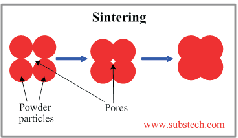
\includegraphics[width=\textwidth]{figures/sinter_2-crop.pdf}
 \end{columns}
 %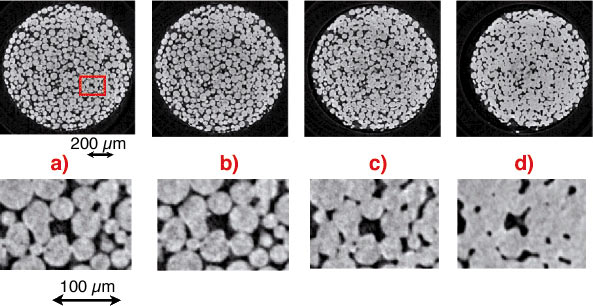
\includegraphics[width=0.6\textwidth]{figures/fig081.jpeg}
\end{center}
\end{frame}


%%%%%%%%%%%%%%%%%%%%%%%%%%%%%%%%%%%%%%%%%%%%%%%%%%%%%%%%%%%%%%%%%%%%%%%%%%%%%%%%%%%%%%%%%%%%%%%%%%%
\begin{frame}
 \frametitle{Constitutive modeling}
 Macroscopic modeling of sintering
 \begin{itemize}
  \item Typically porosity as an internal variable
  \item Complex model structure, requires many parameters --- calibration problem very ill-posed
  \item Selected references: \roughcite{Svoboda \& Riedel (1996)}, \roughcite{Mähler, Ekh \& Runesson (1999)}, \roughcite{Olevsky \& German (1998)}
 \end{itemize}

Mesoscale modeling - deformation driven by surface tension
 \begin{itemize}
  \item Multi-particle sintering
  \item Selected references: \roughcite{Jagota \& Dawson (1988)}, \roughcite{Xu \& Mehrabadi (1997)}, \roughcite{Zhou \& Derby (1998)}, \roughcite{Peric et al.\ (2006-)}, \roughcite{Javili \& Steinmann (2009)}, \roughcite{Pino-Muñoz et al.\ (2013)}
 \end{itemize}

% Computational homogenization - FE\textsuperscript{2}
% \begin{itemize}
%   \item Selected references:  \roughcite{Geers \& al.},  \roughcite{Fish \& al.},
%  \roughcite{Miehe \& al.}, \roughcite{Larsson \& Runesson [adaptive multiscale]}
% \end{itemize}
\end{frame}

%%%%%%%%%%%%%%%%%%%%%%%%%%%%%%%%%%%%%%%%%%%%%%%%%%%%%%%%%%%%%%%%%%%%%%%%%%%%%%%%%%%%%%%%%%%%%%%%%%%
\section{Theory}
% \begin{frame}
%  \frametitle{Surface tension on free surface and interfaces}
% \small
%  \vspace{-1em}
%  \begin{center}
%   \scalebox{0.75}{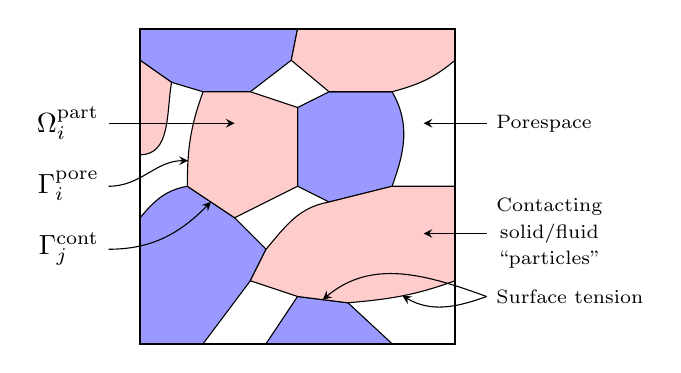
\begin{tikzpicture}[>=stealth,scale=4]
  \coordinate (A) at (0.35,0.2);
  \coordinate (B) at (0.4,0.3);
  \coordinate (C) at (0.3,0.4);
  \coordinate (D) at (0.15,0.5);
  \coordinate (E) at (0.66,0.13);
  \coordinate (F) at (0.6,0.45);
  \coordinate (G) at (0.8,0.5);
  \coordinate (H) at (0.5,0.5);
  \coordinate (I) at (0.5,0.75);
  \coordinate (J) at (0.6,0.8);
  \coordinate (K) at (0.8,0.8);
  \coordinate (L) at (0.35,0.8);
  \coordinate (M) at (0.5,1);
  \coordinate (N) at (0,0.9);
  \coordinate (O) at (0.1,0.83);
  \coordinate (P) at (0.5,0.15);
  \coordinate (Q) at (0.48,0.9);
  \coordinate (R) at (0.2,0.8);
  
  % Region 1 particles 
  \draw[fill=blue!40] 
  (0,0) -- (0.2,0) -- (A) -- (B) -- (C) -- (D) to[out=190,in=50] (0,0.4) -- cycle %A
  (0.4,0) -- (P) -- (E) -- (0.8,0) -- cycle %B
  (F) -- (G) to[out=70,in=-60] (K) -- (J) -- (I) -- (H) -- cycle %C
  (M) -- (Q) -- (L) -- (R) -- (O) -- (N) -- (0,1) -- cycle %D
  ;

  % Region 2 particles
  \draw[fill=red!20]
  (0,0.6) to[out=0,in=-100] (O) -- (N) -- cycle %E
  (D) to[out=90,in=-110] coordinate[near start] (surf3) (R) -- (L) -- (I) -- (H) -- (C) -- (D) coordinate[midway] (surf4) %F
  (M) -- (Q) -- (J) -- (K) to[out=15,in=-140] (1,0.9) -- (1,1) -- cycle %G
  (1,0.2) to[out=-160,in=5] coordinate[midway] (surf1) (E) -- (P) coordinate[midway] (surf2) -- (A) -- (B) to[out=50,in=-170] (F) -- (G) -- (1,0.5) -- cycle %H
  ;

  \draw[thick] (0,0) rectangle (1,1);

  % Annotations
  \draw[<-] (0.9,0.7) -- (1.1,0.7) node[right,font=\scriptsize] {Porespace};
  \draw[<-] (0.9,0.35) -- (1.1,0.35) node[right,font=\scriptsize] {\shortstack{Contacting\\solid/fluid\\``particles''}};
  \draw[<-] (surf1) to[out=-30,in=-160] (1.1,0.15) node[right,font=\scriptsize] {Surface tension};
  \draw[<-] (surf2) to[out=40,in=160] (1.1,0.15); % extra arrow
  \draw[<-] (surf3) to[out=180,in=0] (-0.1,0.5) node[left] {$\Gamma_i^{\mathrm{pore}}$};
  \draw[<-] (surf4) to[out=-135,in=0] (-0.1,0.3) node[left] {$\Gamma_j^{\mathrm{cont}}$};
  \draw[<-] (0.3,0.7) to[out=180,in=0] (-0.1,0.7) node[left] {$\Omega_i^{\mathrm{part}}$};
\end{tikzpicture}}
%   \hspace{0.5em}
%   \scalebox{0.75}{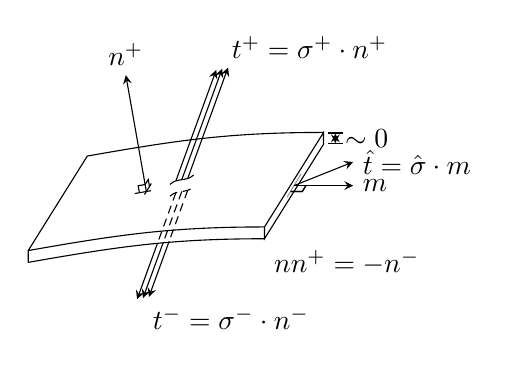
\begin{tikzpicture}[>=stealth,scale=1.5]
 \coordinate (A) at (0,0);
 \coordinate (B) at (2,0.2);
 \coordinate (C) at (2.5,1);
 \coordinate (D) at (0.5,0.8);
 \coordinate (At) at (0,-0.1);
 \coordinate (Bt) at (2,0.1);
 \coordinate (Ct) at (2.5,0.9);

 \draw (A) to[out=10,in=180] (B)
      (At) to[out=10,in=180] (Bt)
      (Bt) -- (B) -- (C) coordinate[midway] (E) -- (Ct) -- cycle
      (At) -- (A) -- (D) to[out=10,in=180] (C);

 % Binormal m
 \draw[draw=black!40] (E)++(0,-0.05)++(-0.06,-0.1) -- +(0.12,0.2);
 \draw[->] (E)++(0,-0.05) -- +(0.5,0) node[right]{$\ta{m}$};
 \draw[->] (E)++(0,-0.05) -- +(0.5,0.2) node[right]{$\hat{\ta{t}}=\hat{\ts{\sigma}}\cdot\ta{m}$};
 \draw (E)++(-0.03,-0.1) -- ++(0.1,0) -- +(0.03,0.05);
 \draw (E)++(0,-0.05)++(-0.03,-0.05) -- ++(0.1,0) -- +(0.03,0.05);

 
 % Normal
 \coordinate (n) at (1,0.5);
 \draw[->] (n) -- +(100:1) node[above]{$\ta{n}^+$};
 \draw (n)++(190:0.06) -- ++(100:0.06) -- +(190:-0.06);
 \draw (n)++(190:0.1) -- +(190:-0.14);
 \draw (n)++(58:0.05) -- ++(100:0.06) -- +(58:-0.05);
 \draw (n)++(58:0.08) -- +(58:-0.11);
 %\draw (n)++(190:0.06) -- ++(58:0.05) -- ++(190:-0.06);
 
 % Traction +
 \draw[->] (1.3,0.6) -- +(70:1) node[above right]{$\ta{t}^+ = \ts{\sigma}^+\cdot\ta{n}^+$};
 \draw[->] (1.35,0.61) -- +(70:1);
 \draw[->] (1.25,0.59) -- +(70:1);
 \draw (1.2,0.56) to[out=45,in=-135] (1.4,0.64);

 % Traction -
 \draw[densely dashed] (1.3,0.5) -- +(-110:0.46) coordinate (tmin); \draw[->] (tmin) -- +(-110:0.5) node[below right]{$\ta{t}^- =  \ts{\sigma}^-\cdot\ta{n}^-$};
 \draw[densely dashed] (1.35,0.51) -- +(-110:0.46) coordinate (tmin); \draw[->] (tmin) -- +(-110:0.5);
 \draw[densely dashed] (1.25,0.49) -- +(-110:0.46) coordinate (tmin); \draw[->] (tmin) -- +(-110:0.5);
 \draw[densely dashed] (1.2,0.46) to[out=45,in=-135] (1.4,0.54);

 % Thickness
 \draw[|<->|] ([xshift=0.1cm]C) -- ([xshift=0.1cm]Ct) node[midway,right] {$\sim 0$};

 % Definition
 \node[right] at (2,-0.1) {$\ta{n} \defeq \ta n^+ = -\ta n^-$};
\end{tikzpicture}}
%  \end{center}
% \vspace{-1em}
% \begin{itemize}
%  \item Equilibrium for tractions on smooth surface/interface segments
% \vspace{-0.7em}
% \begin{align*}
%  \ta t^+ + \ta t^- + \ta t_\surf = \ta 0 \text{ on } \Gamma_i^{\mathrm{pore}} \text{ or } \Gamma_j^{\mathrm{cont}},\quad \ta t_\surf \defeq \hat{\ts\sigma}\cdot\hat{\ta\nabla}
% \end{align*}
% $\hat{\ts\sigma} =$ ``surface stress'' (in tangent plane), $\hat{\ta\nabla} =$ ``surface \rlap{gradient''}
%  \item Particle/pore boundaries $\Gamma_i^{\mathrm{pore}}:\;\;\ta t\defeq \ts\sigma^-\cdot\ta n = \ta t_\surf$
% \item Special case: Isotropic homogeneous surface tension: $\hat{\ts\sigma}=\gamma_\surf \hat{\ta I}$, $\hat{\ts I}\defeq\ts I-\ta n\outerp\ta n$ \vspace{-0.5em}
% \begin{align*}
%  \implies\quad \ta t_\surf = - \kappa \gamma_s \ta n,\quad \kappa \defeq \ta n \cdot \hat{\ta\nabla} \text{ (curvature)}
% \end{align*}
%  %\item \roughcite{Steinmann, Javili \& Steinmann (2009-)}
% \end{itemize}
% \end{frame}

%%%%%%%%%%%%%%%%%%%%%%%%%%%%%%%%%%%%%%%%%%%%%%%%%%%%%%%%%%%%%%%%%%%%%%%%%%%%%%%%%%%%%%%%%%%%%%%%%%%
\begin{frame}
 \frametitle{Fine-scale problem --- Green body}

% The sintering phenomenon on the mesoscale is driven by surface tension on the melted binder, and
% the homogenized effect of the surface tension is the so-called sintering stress.
% From the macroscopic perspective, the specimen (green body) shrinks due to this volumetric sintering stress. In the case of inhomogeneous
% initial density in the green body, the sintering can result in unwanted final deformations.

 \begin{itemize}
  \item Initial state --- ``green body'': Compacted (metal) powder
  %\includegraphics[]{figures/}
  \begin{tikzpicture}
  \node at (0,0) {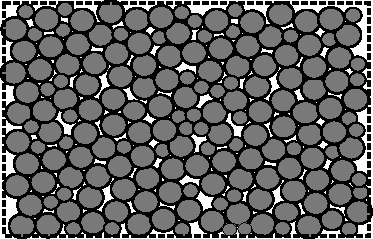
\includegraphics[scale=1.0]{figures/GreenBody.pdf}};
  \draw[latex-] (-2.8,0.1) -- ++(-1,0) node[left] {$\Omega^\particle$};
  \draw[latex-] (-2.8,-0.35) to (-3.8,0.1);
  \draw[-] (3.1,0) -- ++(1,0) node[right] {$\Gamma$};
  \draw[<-] (1.42,0.6) -- (4.1,0.6) node[right] {$\Gamma^\pore$};
  \end{tikzpicture}
  %\caption{Green body with its macroscopic shape as dashed line. Particles are not to scale.}
  \item Particles occupying $\Omega^\particle$ in partial contact
  \item Surface tension acting on internal pore boundaries $\Gamma^\pore$
 \end{itemize}
\end{frame}

%%%%%%%%%%%%%%%%%%%%%%%%%%%%%%%%%%%%%%%%%%%%%%%%%%%%%%%%%%%%%%%%%%%%%%%%%%%%%%%%%%%%%%%%%%%%%%%%%%%
\begin{frame}
 \frametitle{Fine-scale constitutive modeling}
 \begin{itemize}
  \item Quasistatic motion, viscoplastic particles (elastic deformation ignored), spatial setting:
  \begin{align*}
   -[\hat{\ts\sigma}_\dev(\ts d_\dev) - p\ts I]\cdot\ta\nabla &= \ta 0 \text{ in } \Omega^\particle
    \\
    \hat{e}(p) - \ta v\cdot\ta\nabla &= 0\text{ in } \Omega^\particle%, \quad \Omega^\particle = \cup_\alpha \Omega_\alpha^\particle
  \end{align*}
  \item Simplified model $\leadsto$ Stokes' flow.
  \begin{gather*}
   \hat{\ts\sigma}_\dev(\ts d_\dev) \defeq 2\mu {\ts d}_\dev\\
   \hat{\ts\sigma}_\dev(\ts d_\dev) = \ts\sigma + p\ts I,\quad \ts d_\dev \defeq [\ts v\outerp \diff]_\dev^\sym
   \\
   \hat{e}(p) \defeq -C\,p
  \end{gather*}
  \item Subscript $\dev$ denotes deviatoric tensor: $\bullet_\dev = \bullet - \frac13 [\bullet:\ts I]\ts I$
  \item Particles modeled as incompressible viscous flow with large viscosity surrounded by binder with lower viscosity
  \begin{align*}
   \mu^{\mathrm{part}} > \mu^{\mathrm{binder}},\; C = 0\;\text{(only sensible choice)}
  \end{align*}
  %\alert{Note}: Tangent ``stiffness'' $\tf E_{\mathrm{T},\dev}$ from $\dif\ts\sigma_\dev = \tf E_{\mathrm{T},\dev}\dprod \dif\ts d$ used in Newton iterations on subscale (RVE-problem)
 \end{itemize}
\end{frame}

%%%%%%%%%%%%%%%%%%%%%%%%%%%%%%%%%%%%%%%%%%%%%%%%%%%%%%%%%%%%%%%%%%%%%%%%%%%%%%%%%%%%%%%%%%%%%%%%%%%
\begin{frame}
 \frametitle{Surface tension}
\color{gray}
%\begin{figure}[th!]
    \begin{center}
    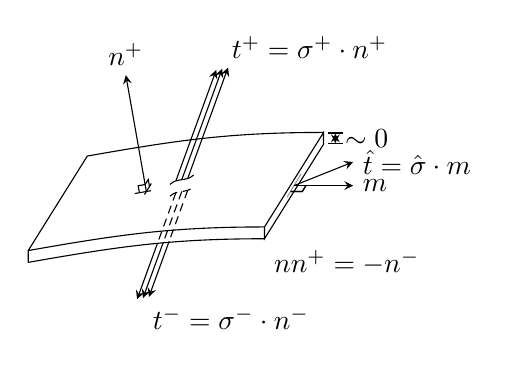
\begin{tikzpicture}[>=stealth,scale=1.5]
 \coordinate (A) at (0,0);
 \coordinate (B) at (2,0.2);
 \coordinate (C) at (2.5,1);
 \coordinate (D) at (0.5,0.8);
 \coordinate (At) at (0,-0.1);
 \coordinate (Bt) at (2,0.1);
 \coordinate (Ct) at (2.5,0.9);

 \draw (A) to[out=10,in=180] (B)
      (At) to[out=10,in=180] (Bt)
      (Bt) -- (B) -- (C) coordinate[midway] (E) -- (Ct) -- cycle
      (At) -- (A) -- (D) to[out=10,in=180] (C);

 % Binormal m
 \draw[draw=black!40] (E)++(0,-0.05)++(-0.06,-0.1) -- +(0.12,0.2);
 \draw[->] (E)++(0,-0.05) -- +(0.5,0) node[right]{$\ta{m}$};
 \draw[->] (E)++(0,-0.05) -- +(0.5,0.2) node[right]{$\hat{\ta{t}}=\hat{\ts{\sigma}}\cdot\ta{m}$};
 \draw (E)++(-0.03,-0.1) -- ++(0.1,0) -- +(0.03,0.05);
 \draw (E)++(0,-0.05)++(-0.03,-0.05) -- ++(0.1,0) -- +(0.03,0.05);

 
 % Normal
 \coordinate (n) at (1,0.5);
 \draw[->] (n) -- +(100:1) node[above]{$\ta{n}^+$};
 \draw (n)++(190:0.06) -- ++(100:0.06) -- +(190:-0.06);
 \draw (n)++(190:0.1) -- +(190:-0.14);
 \draw (n)++(58:0.05) -- ++(100:0.06) -- +(58:-0.05);
 \draw (n)++(58:0.08) -- +(58:-0.11);
 %\draw (n)++(190:0.06) -- ++(58:0.05) -- ++(190:-0.06);
 
 % Traction +
 \draw[->] (1.3,0.6) -- +(70:1) node[above right]{$\ta{t}^+ = \ts{\sigma}^+\cdot\ta{n}^+$};
 \draw[->] (1.35,0.61) -- +(70:1);
 \draw[->] (1.25,0.59) -- +(70:1);
 \draw (1.2,0.56) to[out=45,in=-135] (1.4,0.64);

 % Traction -
 \draw[densely dashed] (1.3,0.5) -- +(-110:0.46) coordinate (tmin); \draw[->] (tmin) -- +(-110:0.5) node[below right]{$\ta{t}^- =  \ts{\sigma}^-\cdot\ta{n}^-$};
 \draw[densely dashed] (1.35,0.51) -- +(-110:0.46) coordinate (tmin); \draw[->] (tmin) -- +(-110:0.5);
 \draw[densely dashed] (1.25,0.49) -- +(-110:0.46) coordinate (tmin); \draw[->] (tmin) -- +(-110:0.5);
 \draw[densely dashed] (1.2,0.46) to[out=45,in=-135] (1.4,0.54);

 % Thickness
 \draw[|<->|] ([xshift=0.1cm]C) -- ([xshift=0.1cm]Ct) node[midway,right] {$\sim 0$};

 % Definition
 \node[right] at (2,-0.1) {$\ta{n} \defeq \ta n^+ = -\ta n^-$};
\end{tikzpicture}
    %\caption{Thin shell representing a surface with in-plane forces due to ``surface tension''.}
    %%\label{fig:surfacestress}
    \end{center}
%\end{figure}
% A vital part of the simulation is the modeling of surface tension, which acts as the ``driving force'' for liquid-phase sintering.
% An extensive theory on boundary energy potentials has been developed by Steinmann \cite{steinmann_boundary_2008}, which has served as the basis for the surface tension modeling in this work.
% In short; equilibrium across a surface $\mathcal{S}$ represented by a thin shell bounded by the curve $\mathcal{C}$, as in \figref{fig:surfacestress}, can be stated as:
\begin{itemize}
\color{gray}
 \item Equilibrium:
 \vspace{-2em}
\begin{align*}
    \ta{t}^+ + \ta{t}^- + \ta{t}_\surf &= \ta{0} \quad \text{on} \,\, \mathcal{S} \quad \text{with } \ta{t}_\surf \defeq \hat{\ts\sigma}\cdot\hat{\diff}
%\label{eq103KR}
% \\
%     \sum_i \hat{\ta t}_i &= \ta{0} \quad \text{on} \,\, \mathcal{C}
%%\label{eq104KR}
\end{align*}
\item Surface gradient: $\hat\diff \defeq \diff - [\diff\cdot\ta n]\ta n$
\color{black}
\item Isotropy: $\hat{\ts\sigma} = \gamma_\surf[\ts I-\ta n\outerp\ts n]$ $\implies$
$ \ta t_\surf = -\kappa \gamma_\surf \ta n$, where $\kappa \defeq \ta n \cdot\hat{\diff}$
\item $\gamma_\surf = $ surface energy = ``surface tension''
\end{itemize}
\end{frame}

%%%%%%%%%%%%%%%%%%%%%%%%%%%%%%%%%%%%%%%%%%%%%%%%%%%%%%%%%%%%%%%%%%%%%%%%%%%%%%%%%%%%%%%%%%%%%%%%%%%
\begin{frame}
 \frametitle{Weak form of ``fine-scale'' problem}
%\footnotesize
 \begin{itemize}
  \item Sintering particles occupying domain $\Omega^\particle$ with internal pore boundary $\Gamma^\pore$:
Find $(\ta v,p)\in \set V \times \set P$ such that
\begin{align*}
  \int_{\mathrlap{\Omega^\particle}} \;[\hat{\ts\sigma}_\dev([\ta v\outerp\diff]_\dev^\sym)-p\ts I]\dprod[\delta\ta v\outerp\ta\nabla]\dif v &=
   \int_{\mathrlap{\Gamma^\pore}} \;\gamma_\surf[\delta\ta v\cdot\hat{\ta\nabla}] \dif a
    % +\int_{\mathrlap{\Gamma_\Neumann^\external}} \;\ta t_p\cdot\delta\ta v\dif a \; 
    && \forall \delta \ta v\in \set V^0
\\
  \int_{\mathrlap{\Omega^\particle}} \;[\hat{e}(p) - \ta v\cdot\ta\nabla]\delta p \dif v &= 0 && \forall \delta p\in \set P
\end{align*}
%\alert{Note}: Obtained via use of surface divergence theorem + equilibrium for singular curves $C_i$

 %\item \alert{Surface tension}: Stems from the surface potential, defined by $\gamma_\surf$.
 \item Explicit time-stepping
 \item \alert{Remark}: Incompressible elasticity in Paper C: replace $\ta v \to \ta u$
 \item \alert{Remark}: Too many particles for Direct Numerical Simulation (DNS) $\leadsto$ homogenization
 \end{itemize}
\end{frame}


%%%%%%%%%%%%%%%%%%%%%%%%%%%%%%%%%%%%%%%%%%%%%%%%%%%%%%%%%%%%%%%%%%%%%%%%%%%%%%%%%%%%%%%%%%%%%%%%%%%
\begin{frame}
 \frametitle{Two-scale problem: FE\textsuperscript{2}}

\begin{itemize}
\item Variationally Consistent Homogenization (VCH) of fine-scale problem
\scalebox{0.75}{
\begin{tikzpicture}[scale=1.0]
 \node at (0,0) {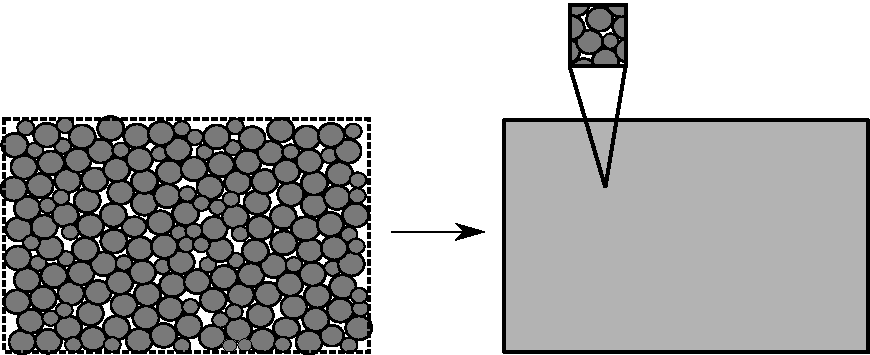
\includegraphics[scale=0.6]{figures/Homogenization}};
 \draw[-] (1.35,1.5) -- +(-0.5,0) node[left] {$\Omega_\rve$};
 \node[right] at (2.1,1.5) {Representative Volume Element (RVE)};
 \node at (-2.5,-2.2) {Fine-scale};
 \node at (2.5,-2.2) {Macroscale};
 \node at (0,0) {VCH};
 \draw[latex-] (-4.1,0.1) -- ++(-1,0) node[left] {$\Omega^\particle$};
 \draw[latex-] (-4.2,-0.15) to (-5.1,0.1);
 \draw[latex-] (4.4,0) -- ++(1,0) node[right] {$\Gamma^\Neumann$, $\Gamma^\Dirichlet$};
 \node at (2.5,-0.5) {$\Omega$};
 \draw[very thick] (-3.7,-.3) rectangle +(0.5,0.5);
 \draw[] (-3.45,.2) |- (0,1.5);
\end{tikzpicture}
}
\item Numerical solution: FE\textsuperscript{2}

\item Idealized RVE consisting of a single unit cell of spherical particles in contact
\begin{center}
\scalebox{0.75}{
\begin{tikzpicture}[scale=1.0]
 \node at (0,0) {
\includegraphics[scale=0.15]{figures/initial_rve}};
 \node at (-0.75,0.85) {$\Omega_\rve^\particle$};
 \draw[latex-] (-1.33,0.) -- ++(-1,0) node[left] {$\Gamma_\rve$};
 \draw[latex-] (45:0.5) -- +(1.6,0.5) node[right] {$\Gamma_\rve^\pore \defeq \Omega_\rve \cap \Gamma^\pore$};
 \node[right] at (1.9536,0) {$\Omega_\rve^\particle \defeq \Omega_\rve \cap \Omega^\particle$};
\end{tikzpicture}
}
\end{center}
\end{itemize}
\end{frame}


%%%%%%%%%%%%%%%%%%%%%%%%%%%%%%%%%%%%%%%%%%%%%%%%%%%%%%%%%%%%%%%%%%%%%%%%%%%%%%%%%%%%%%%%%%%%%%%%%%%
\begin{frame}
 \frametitle{Variationally Consistent Homogenization}
\begin{itemize}
 \item Volume average operators over the RVE-window $\Omega_\rve$
\begin{align*}
 \homgen{\bullet} \defeq \frac{1}{\volume} \int_{\Omega_\rve^\particle} \bullet \dif V%,\quad \Omega_\rve^\particle \defeq \Omega_\rve \cap \Omega^\particle
\\
 \shomgen{\bullet} \defeq \frac{1}{\volume} \int_{\Gamma^\pore_\rve} \bullet \dif S%,\quad \Gamma^\pore_\rve \defeq \Omega_\rve \cap \Gamma^\pore
\end{align*}
 \item Decompose the fields into macroscopic and fluctuating parts:
 \begin{align*}
  \ta v = \ta v^\macro + \ta v^\fluct
   \\
  p = p^\macro + p^\fluct
 \end{align*}
 \item Variationally Consistent Homogenization $\leadsto$ macroscale problem
\end{itemize}
\end{frame}


%%%%%%%%%%%%%%%%%%%%%%%%%%%%%%%%%%%%%%%%%%%%%%%%%%%%%%%%%%%%%%%%%%%%%%%%%%%%%%%%%%%%%%%%%%%%%%%%%%%
%%%%%%%%%%%%%%%%%%%%%%%%%%%%%%%%%%%%%%%%%%%%%%%%%%%%%%%%%%%%%%%%%%%%%%%%%%%%%%%%%%%%%%%%%%%%%%%%%%%
%%%%%%%%%%%%%%%%%%%%%%%%%%%%%%%%%%%%%%%%%%%%%%%%%%%%%%%%%%%%%%%%%%%%%%%%%%%%%%%%%%%%%%%%%%%%%%%%%%%
%%%%%%%%%%%%%%%%%%%%%%%%%%%%%%%%%%%%%%%%%%%%%%%%%%%%%%%%%%%%%%%%%%%%%%%%%%%%%%%%%%%%%%%%%%%%%%%%%%%
%%%%%%%%%%%%%%%%%%%%%%%%%%%%%%%%%%%%%%%%%%%%%%%%%%%%%%%%%%%%%%%%%%%%%%%%%%%%%%%%%%%%%%%%%%%%%%%%%%%
%%%%%%%%%%%%%%%%%%%%%%%%%%%%%%%%%%%%%%%%%%%%%%%%%%%%%%%%%%%%%%%%%%%%%%%%%%%%%%%%%%%%%%%%%%%%%%%%%%%


\section{Paper}
%%%%%%%%%%%%%%%%%%%%%%%%%%%%%%%%%%%%%%%%%%%%%%%%%%%%%%%%%%%%%%%%%%%%%%%%%%%%%%%%%%%%%%%%%%%%%%%%%%%
%%%%%%%%%%%%%%%%%%%%%%%%%%%%%%%%%%%%%%%%%%%%%%%%%%%%%%%%%%%%%%%%%%%%%%%%%%%%%%%%%%%%%%%%%%%%%%%%%%%   A
%%%%%%%%%%%%%%%%%%%%%%%%%%%%%%%%%%%%%%%%%%%%%%%%%%%%%%%%%%%%%%%%%%%%%%%%%%%%%%%%%%%%%%%%%%%%%%%%%%%
\subsection{A}
\begin{frame}
 \frametitle{Paper A}
\begin{center}
 %\fullcite{ohman_computational_2012}
Mikael Öhman, Kenneth Runesson, and Fredrik Larsson.
\\[1em]
\textit{Computational mesoscale modeling and homogenization of liquid-phase sintering of particle agglomerates}.
\\[1em]
Technische Mechanik \textbf{32} (2012), 463--483. \textsc{issn}: 0232-3869.
\end{center}
\end{frame}

%%%%%%%%%%%%%%%%%%%%%%%%%%%%%%%%%%%%%%%%%%%%%%%%%%%%%%%%%%%%%%%%%%%%%%%%%%%%%%%%%%%%%%%%%%%%%%%%%%%
\begin{frame}
 \frametitle{Choice of prolongation}
\begin{itemize}
 \item First order Taylor expansion of the velocity, and no macroscale pressure
\begin{align*}
 \ta v^\macro &= \bar{\ta v} + [\bar{\ta v}\outerp\diff]\cdot[\ta x - \bar{\ta x}]
\\
 p^\macro &= 0
\end{align*}
\item Constraint on the fluctuation $\ta v^\fluct$ within each RVE via the condition
\begin{align*}
 \frac{1}{\volume} \int_{\Gamma_\rve} \ta v\outerp\ta n \dif S &= \bar{\ta v}\outerp\diff
\end{align*}
\item \textbf{Remark}: $\bar{\ta v}\outerp\diff$ represents the ``effective'' volume average for a porous domain
\end{itemize}
\end{frame}

%%%%%%%%%%%%%%%%%%%%%%%%%%%%%%%%%%%%%%%%%%%%%%%%%%%%%%%%%%%%%%%%%%%%%%%%%%%%%%%%%%%%%%%%%%%%%%%%%%%
\begin{frame}
 \frametitle{Macroscale problem}
\begin{itemize}
 \item Find $\bar{\ta v} \in \bar{\set V}$ such that
 \begin{align*}
  \int_\Omega \highlight{\bar{\ts\sigma}\{\bar{\ts d}\}}\dprod[\delta\bar{\ta v}\outerp\diff]\dif V = 0\quad \forall \delta\bar{\ta v} \in \bar{\set{V}}^0
 \end{align*}
 \item RVE-input: $\bar{\ts d} \defeq [\bar{\ta v}\outerp\diff]^\sym$
 \item Homogenized stress identified as
 \begin{align*}
  \bar{\ts\sigma} \defeq \frac{1}{\volume} \int_{\Gamma_\rve} \ta t \outerp [\ta x-\bar{\ta x}]\dif S
 \end{align*}
 \item Standard RVE-problem (Dirichlet boundary condition)
 \item \textbf{Remark}: ``Displacement'' formulation valid only for macroscopic compressibility
\end{itemize}
\end{frame}

%%%%%%%%%%%%%%%%%%%%%%%%%%%%%%%%%%%%%%%%%%%%%%%%%%%%%%%%%%%%%%%%%%%%%%%%%%%%%%%%%%%%%%%%%%%%%%%%%%%
\begin{frame}
 \frametitle{Paper A summarized}
\begin{center}
 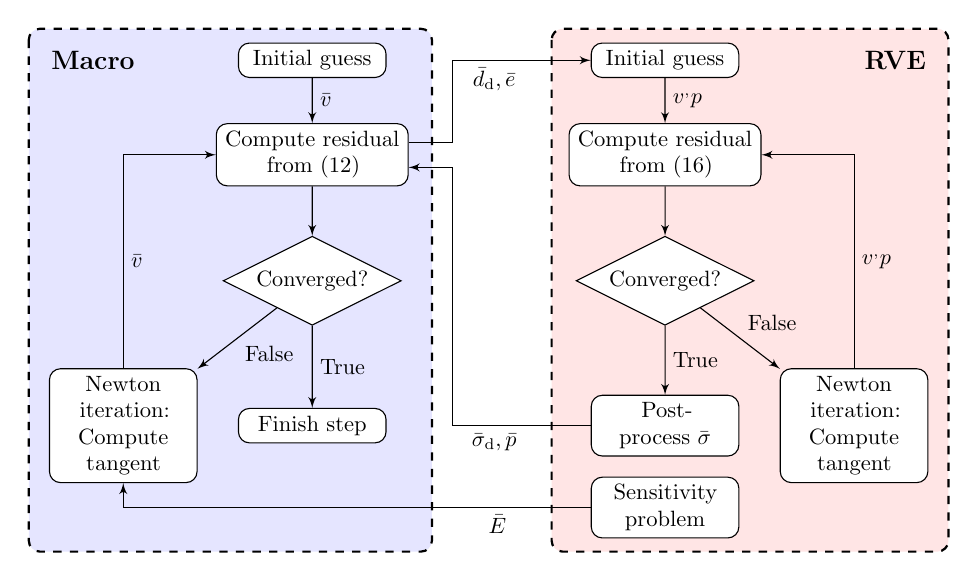
\begin{tikzpicture}[node distance = 2cm, auto,scale=0.8, transform shape, >=latex']
    %\small
    %\tikzstyle{every node}=[font=\footnotesize]
    \tikzstyle{group}    = [rectangle, draw, thick, dashed, text width=6em, text centered, rounded corners]
    \tikzstyle{decision} = [diamond,   draw, fill=white, aspect=2, node distance=2.5cm, inner sep=2pt]
    \tikzstyle{block}    = [rectangle, draw, fill=white, text width=6em, text centered, rounded corners]
    \tikzstyle{line}     = [draw, ->]

    \draw [thick, dashed, fill=blue!10, rounded corners] (-4.5,0.5) rectangle ( 1.9,-7.8);
    \draw [thick, dashed, fill=red!10,  rounded corners] ( 3.8,0.5) rectangle (10.1,-7.8);
    \node [below right, inner sep=10pt] at (-4.5,0.5) { \textbf{\large Macro} };
    \node [below left,  inner sep=10pt] at (10.1,0.5) { \textbf{\large RVE} };

    % Place nodes
    \node [block] (init) {Initial guess};
    \node [block, below of=init, text width=8em, node distance=1.5cm] (residual) {Compute residual from (12)};
    \node [decision, below of=residual,node distance=2cm] (convergence) {Converged?};
    \node [block, below of=convergence, node distance=2.3cm] (stop) {Finish step};
    \node [block, left of=stop, node distance=3cm] (update) {Newton iteration: Compute tangent};
    % Draw edges
    \path [line] (init) -- (residual) node[midway] {$\bar{\ta{v}}$};
    \path [line] (residual) -- (convergence);
    \path [line] (convergence) -- node {False} (update);
    \path [line] (convergence) -- node {True} (stop);
    \path [line] (update) |- node[near start,right] {$\bar{\ta{v}}$} (residual);

    % Place nodes
    \node [block, right of=init, node distance=5.6cm] (rve_init) {Initial guess};
    \node [block, below of=rve_init, text width=8em, node distance=1.5cm] (rve_residual) {Compute residual from (16)};
    \node [decision, below of=rve_residual, node distance=2cm] (rve_convergence) {Converged?};
    \node [block, below of=rve_convergence, node distance=2.3cm] (rve_stop) {Post-process $\bar{\ts\sigma}$};
    \node [block, right of=rve_stop, node distance=3cm] (rve_update) {Newton iteration: Compute tangent};
    % Sensitivity problem
    \node [block, below of=rve_stop, node distance=1.3cm] (rve_sensitivity) {Sensitivity problem};
    
    % Draw edges
    \path [line] (rve_init) -- (rve_residual) node[midway] {$\ta{v}^\fluct,p$};
    \path [line] (rve_residual) -- (rve_convergence);
    \path [line] (rve_convergence) -- node {False} (rve_update);
    \path [line] (rve_convergence) -- node {True} (rve_stop);
    \path [line] (rve_update) |- node[right, near start] {$\ta{v}^\fluct,p$} (rve_residual);

    \path [line] (residual.east) ++(0, 0.2cm) -- ++(0.7cm,0) |- node [below,pos=0.65] {$\bar{\ts d}_\dev, \bar{e}$} (rve_init);
    % Draw this backwards in order to get exact alignments
    \path [line, <-] (residual.east) ++(0,-0.2cm) -- ++(0.7cm,0) |- node [below,pos=0.65] {$\bar{\ts\sigma}_\dev, \bar{p}$} (rve_stop);

    \path [line] (rve_sensitivity) -| node[below, pos=0.10] {$\bar{\tf E}$} (update);
\end{tikzpicture}

\end{center}
\end{frame}



%%%%%%%%%%%%%%%%%%%%%%%%%%%%%%%%%%%%%%%%%%%%%%%%%%%%%%%%%%%%%%%%%%%%%%%%%%%%%%%%%%%%%%%%%%%%%%%%%%%
%%%%%%%%%%%%%%%%%%%%%%%%%%%%%%%%%%%%%%%%%%%%%%%%%%%%%%%%%%%%%%%%%%%%%%%%%%%%%%%%%%%%%%%%%%%%%%%%%%%   B
%%%%%%%%%%%%%%%%%%%%%%%%%%%%%%%%%%%%%%%%%%%%%%%%%%%%%%%%%%%%%%%%%%%%%%%%%%%%%%%%%%%%%%%%%%%%%%%%%%%
\subsection{B}
\begin{frame}
 \frametitle{Paper B}
\begin{center}
 %\fullcite{ohman_computational_2013}
Mikael Öhman, Kenneth Runesson, and Fredrik Larsson.
\\[1em]
\textit{Computational homogenization of liquid-phase sintering with seamless transition from
macroscopic compressibility to incompressibility}.
\\[1em]
Computer Methods in Applied Mechanics and Engineering \textbf{266} (2013), 219--228. \textsc{issn}: 0045-7825.
\textsc{doi}: 10.1016/j.cma.2013.07.006
\end{center}
\end{frame}

%%%%%%%%%%%%%%%%%%%%%%%%%%%%%%%%%%%%%%%%%%%%%%%%%%%%%%%%%%%%%%%%%%%%%%%%%%%%%%%%%%%%%%%%%%%%%%%%%%%
\begin{frame}
 \frametitle{Macroscale problem}
\begin{itemize}
 \item When an RVE has no pores left, it is no longer possible to control the volumetric part of the deformation
\begin{center}
  \begin{tikzpicture}
   \node at (0,0) {\includegraphics[width=0.5\linewidth]{figures/DeformationModes}};
   \draw[opacity=0.5,line width=3pt,red] (-2.1,0) circle (1) (-2.1,0)+(135:1) -- +(-45:1);
%    \node at (2,-1) {OK};
%    \node at (0,-1) {OK};
%    \node at (-2,-1) {Not OK};
  \end{tikzpicture}
\end{center}

%  \item Switch control variables
%   \begin{align*}
%    \bar{\ts d} &\rightarrow \bar{\ts\sigma}
%    \\
%     &\equiv
%    \\
%    (\bar{\ts d}_\dev, \bar{e}) &\rightarrow (\bar{\ts\sigma}_\dev, \bar{p})
%    \\
%    &\leadsto
%    \\
%    (\bar{\ts d}_\dev, \bar{p}) &\rightarrow (\bar{\ts\sigma}_\dev, \bar{e})
%   \end{align*}

 \item Constraint on the volumetric part of the deformation within each RVE via the weak condition
\begin{align*}
 -\int_\Omega \delta\bar{p} \ts I \dprod \left[\frac{1}{\volume} \int_{\Gamma_\rve} \ta v\outerp\ta n \dif S - \bar{\ta v}\outerp\diff\right] \dif V &= 0\quad\forall\;\delta\bar{p}\in\bar{\set P}
\end{align*}
\item Switch of control variables: $\bar{\ts d} \to (\bar{\ts d}_\dev, \bar{p})$
\end{itemize}
\end{frame}

%%%%%%%%%%%%%%%%%%%%%%%%%%%%%%%%%%%%%%%%%%%%%%%%%%%%%%%%%%%%%%%%%%%%%%%%%%%%%%%%%%%%%%%%%%%%%%%%%%%
\begin{frame}
 \frametitle{Macroscale problem}
\begin{itemize}
 \item Find $(\bar{\ta v}, \bar{p}) \in \bar{\set V}\times\bar{\set P}$ such that
 \begin{align*}
  \int_\Omega [\highlight{\bar{\ts\sigma}_\dev\{\bar{\ts d}_\dev, \bar{p}\}} - \bar{p}\ts I]\dprod[\delta\bar{\ta v}\outerp\diff]\dif V &= 0\quad \forall \delta\bar{\ta v} \in \bar{\set{V}}^0
\\
  \int_\Omega [-\bar{\ta v}\cdot\diff + \highlight{\bar{e}\{\bar{\ts d}_\dev, \bar{p}\}}]\delta\bar{p}\dif V &= 0\quad \forall \delta\bar{p} \in \bar{\set{P}}
 \end{align*}
 \item RVE-input: $\bar{\ts d}_\dev\defeq [\bar{\ta v}\outerp\diff]^\sym_\dev$ and $\bar{p}$.
 \item Homogenized response variables identified as
 \begin{align*}
 \bar{\ts\sigma}_\dev &\defeq \frac{1}{\volume} \left[\int_{\Gamma_\rve} \ta t \outerp [\ta x-\bar{\ta x}]\dif S\right]_\dev
\\
 \bar{e} &\defeq \frac{1}{\volume} \int_{\Gamma_\rve} \ta v \cdot \ta n\dif S
 \end{align*}
\end{itemize}
\end{frame}

%%%%%%%%%%%%%%%%%%%%%%%%%%%%%%%%%%%%%%%%%%%%%%%%%%%%%%%%%%%%%%%%%%%%%%%%%%%%%%%%%%%%%%%%%%%%%%%%%%%
\begin{frame}
 \frametitle{RVE problem --- Dirichlet b.c.}
\begin{itemize}
 \item For given macroscale variables $\bar{\ts d}_\dev$ and $\bar{p}$, find ($\ta{v}^\fluct,p,\bar{e})\in\set{V}_\rve^{0}\times\set{P}_\rve\times\set{R}$ that solve the system
%----------------------------------------------------------------------------
\begin{flalign*}
 \int_{\mathrlap{\Omega_\rve^\particle}} [\hat{\ts\sigma}_\dev(\highlight{\bar{\ts d}_\dev} + [\ta v^\fluct \outerp\diff]^\sym_\dev)-p\ts I]\dprod[\delta\ta v^\fluct \outerp\diff] \dif V = \int_{\mathrlap{\Gamma_\rve^\pore}} \gamma_\surf [\delta\ta v^\fluct\cdot\hat{\diff}] \dif S
\end{flalign*}
\vspace{-2em}
\begin{flalign*}
&&
 \forall\;\delta\ta v^\fluct \in \set V_\rve^0
% \end{flalign*}
\\
% \begin{flalign*}
 \int_{\mathrlap{\Omega_\rve^\particle}} -\delta p[\bar{e} + \delta\ta v^\fluct \outerp\diff] \dif V &= 0
%\\
&
  \forall\;\delta p \in \set P_\rve
% \end{flalign*}
\\
% \begin{flalign*}
 \int_{\mathrlap{\Omega_\rve^\particle}} -p \dif V \delta\bar{e} &= \left[\int_{\Gamma_\rve^\pore} \frac23 \gamma_\surf \dif S - \highlight{\bar{p}}\right] \delta\bar{e}
%\\
&
  \forall\;\delta\bar{e} \in \set R
\end{flalign*}
 \item In practice: Solve with standard $(\ta v,p)$-formulation and specialized boundary condition that includes $\bar{e}$.
\end{itemize}
\end{frame}

%%%%%%%%%%%%%%%%%%%%%%%%%%%%%%%%%%%%%%%%%%%%%%%%%%%%%%%%%%%%%%%%%%%%%%%%%%%%%%%%%%%%%%%%%%%%%%%%%%%
\begin{frame}
 \frametitle{Paper B summarized}
\begin{center}
 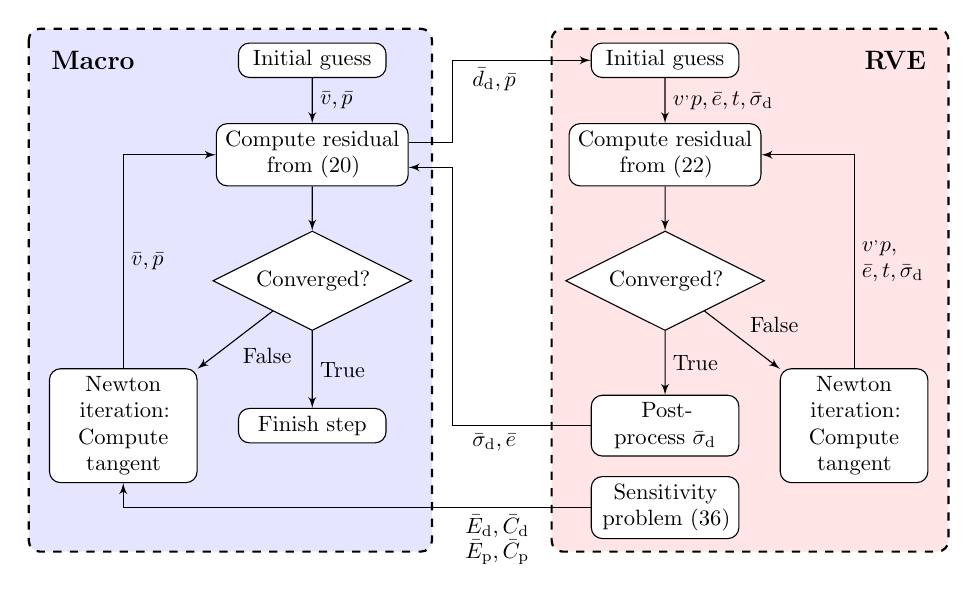
\begin{tikzpicture}[node distance = 2cm, auto,scale=0.8, transform shape, >=latex']
    %\small
    %\tikzstyle{every node}=[font=\footnotesize]
    \tikzstyle{group}    = [rectangle, draw, thick, dashed, text width=6em, text centered, rounded corners]
    \tikzstyle{decision} = [diamond,   draw, fill=white, text width=6em, text centered, aspect=2, node distance=2.5cm, inner sep=2pt]
    \tikzstyle{block}    = [rectangle, draw, fill=white, text width=6em, text centered, rounded corners]
    \tikzstyle{line}     = [draw, ->]

    \draw [thick, dashed, fill=blue!10, rounded corners] (-4.5,0.5) rectangle ( 1.9,-7.8);
    \draw [thick, dashed, fill=red!10,  rounded corners] ( 3.8,0.5) rectangle (10.1,-7.8);
    \node [below right, inner sep=10pt] at (-4.5,0.5) { \textbf{\large Macro} };
    \node [below left,  inner sep=10pt] at (10.1,0.5) { \textbf{\large RVE} };

    % Place nodes
    \node [block] (init) {Initial guess};
    \node [block, below of=init, text width=8em, node distance=1.5cm] (residual) {Compute residual from (20)};
    \node [decision, below of=residual,node distance=2cm] (convergence) {Converged?};
    \node [block, below of=convergence, node distance=2.3cm] (stop) {Finish step};
    \node [block, left of=stop, node distance=3cm] (update) {Newton iteration: Compute tangent};
    % Draw edges
    \path [line] (init) -- (residual) node[midway] {$\bar{\ta{v}},\bar{p}$};
    \path [line] (residual) -- (convergence);
    \path [line] (convergence) -- node {False} (update);
    \path [line] (convergence) -- node {True} (stop);
    \path [line] (update) |- node[near start,right] {$\bar{\ta{v}},\bar{p}$} (residual);

    % Place nodes
    \node [block, right of=init, node distance=5.6cm] (rve_init) {Initial guess};
    \node [block, below of=rve_init, text width=8em, node distance=1.5cm] (rve_residual) {Compute residual from (22)};
    \node [decision, below of=rve_residual, node distance=2cm] (rve_convergence) {Converged?};
    \node [block, below of=rve_convergence, node distance=2.3cm] (rve_stop) {Post-process $\bar{\ts\sigma}_\dev$};
    \node [block, right of=rve_stop, node distance=3cm] (rve_update) {Newton iteration: Compute tangent};
    % Sensitivity problem
    \node [block, below of=rve_stop, node distance=1.3cm] (rve_sensitivity) {Sensitivity problem (36)};
    
    % Draw edges
    \path [line] (rve_init) -- (rve_residual) node[midway] {$\ta{v}^\fluct,p, \bar{e}, \ta t, \bar{\ts\sigma}_\dev$};
    \path [line] (rve_residual) -- (rve_convergence);
    \path [line] (rve_convergence) -- node {False} (rve_update);
    \path [line] (rve_convergence) -- node {True} (rve_stop);
    \path [line] (rve_update) |- node[right, near start, text width=1.5em] {$\ta{v}^\fluct,p$, $\bar{e}, \ta t, \bar{\ts\sigma}_\dev$} (rve_residual);

    \path [line] (residual.east) ++(0, 0.2cm) -- ++(0.7cm,0) |- node [below,pos=0.65] {$\bar{\ts d}_\dev, \bar{p}$} (rve_init);
    % Draw this backwards in order to get exact alignments
    \path [line, <-] (residual.east) ++(0,-0.2cm) -- ++(0.7cm,0) |- node [below,pos=0.65] {$\bar{\ts\sigma}_\dev, \bar{e}$} (rve_stop);

    \path [line] (rve_sensitivity) -| node[below, pos=0.10] {$\substack{\displaystyle\bar{\tf E}_\ded,\bar{\ts C}_\ded \\ \displaystyle\bar{\ts E}_\dep,\bar{C}_\dep}$} (update);
\end{tikzpicture}

\end{center}
\end{frame}

%%%%%%%%%%%%%%%%%%%%%%%%%%%%%%%%%%%%%%%%%%%%%%%%%%%%%%%%%%%%%%%%%%%%%%%%%%%%%%%%%%%%%%%%%%%%%%%%%%%
\begin{frame}
 \frametitle{FE\textsuperscript{2} with macroscopic incompressibility}
\begin{center}
 \movie[width=\linewidth,poster]{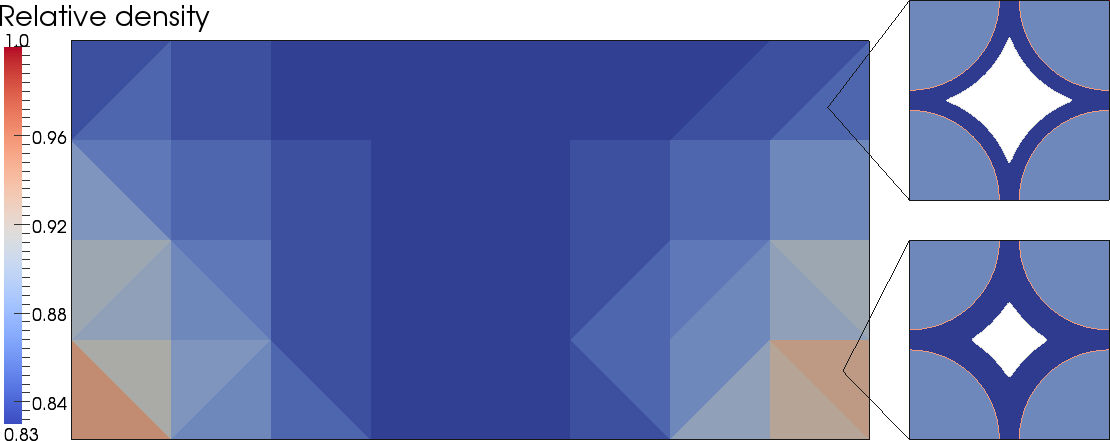
\includegraphics[width=\linewidth]{figures/macro_fe2_0000}}{macro_fe2_slow.wmv}
\end{center}
 \begin{itemize}
  \item Large topological changes $\leadsto$ surface tracking and remeshing required
 \end{itemize}
\end{frame}




%%%%%%%%%%%%%%%%%%%%%%%%%%%%%%%%%%%%%%%%%%%%%%%%%%%%%%%%%%%%%%%%%%%%%%%%%%%%%%%%%%%%%%%%%%%%%%%%%%%
%%%%%%%%%%%%%%%%%%%%%%%%%%%%%%%%%%%%%%%%%%%%%%%%%%%%%%%%%%%%%%%%%%%%%%%%%%%%%%%%%%%%%%%%%%%%%%%%%%%   C
%%%%%%%%%%%%%%%%%%%%%%%%%%%%%%%%%%%%%%%%%%%%%%%%%%%%%%%%%%%%%%%%%%%%%%%%%%%%%%%%%%%%%%%%%%%%%%%%%%%
\subsection{C}
\begin{frame}
 \frametitle{Paper C}
\begin{center}
 %\fullcite{ohman_variationally_2014}
Mikael Öhman, Kenneth Runesson, and Fredrik Larsson.
\\[1em]
\textit{On the variationally consistent computational homogenization of elasticity in the incompressible limit}.
\\[1em]
Advanced Modeling and Simulation in Engineering Sciences (2014). Submitted
\end{center}
\end{frame}

%%%%%%%%%%%%%%%%%%%%%%%%%%%%%%%%%%%%%%%%%%%%%%%%%%%%%%%%%%%%%%%%%%%%%%%%%%%%%%%%%%%%%%%%%%%%%%%%%%%
\begin{frame}
 \frametitle{Choice of prolongation}
\begin{itemize}
 \item First order Taylor expansion of the displacement, and zeroth order expansion of the pressure
\begin{align*}
 \ta u^\macro &= \bar{\ta u} + [\bar{\ta u}\outerp\diff]\cdot[\ta x - \bar{\ta x}]
\\
 p^\macro &= \bar{p}
\end{align*}
 \item Constraints on the fluctuations $\ta u^\fluct$ and $p^\fluct$ within each RVE via the conditions
\begin{align*}
 \homgen{\ta u\outerp\diff} &= \bar{\ta u}\outerp\diff
\\
 \homgen{p} &= \bar{p}
\end{align*}
\end{itemize}
\end{frame}

%%%%%%%%%%%%%%%%%%%%%%%%%%%%%%%%%%%%%%%%%%%%%%%%%%%%%%%%%%%%%%%%%%%%%%%%%%%%%%%%%%%%%%%%%%%%%%%%%%%
\begin{frame}
 \frametitle{Macroscale problem}
\begin{itemize}
 \item Identical macroscale problem to that of Paper B ($\ta v\leadsto\ta u$)
 \color{gray}
 \item Find $(\bar{\ta u}, \bar{p}) \in \bar{\set U}\times \bar{\set P}$ such that
 \begin{align*}
  \int_\Omega [{\bar{\ts\sigma}_\dev\{\bar{\ts\epsilon}_\dev, \bar{p}\}} - \bar{p}\ts I]\dprod[\delta\bar{\ta u}\outerp\diff]\dif V &= 0\quad \forall \delta\bar{\ta u} \in \bar{\set{U}}^0
\\
  \int_\Omega [-\bar{\ta u}\cdot\diff + {\bar{e}\{\bar{\ts\epsilon}_\dev, \bar{p}\}}]\delta\bar{p}\dif V &= 0\quad \forall \delta\bar{p} \in \bar{\set{P}}
 \end{align*}
 \item RVE-input: $\bar{\ts\epsilon}_\dev\defeq [\bar{\ta u}\outerp\diff]^\sym_\dev$ and $\bar{p}$.
 \item Homogenized response variables identified as
 \begin{align*}
 \bar{\ts\sigma}_\dev &\defeq \frac{1}{\volume} \left[\int_{\Gamma_\rve} \ta t \outerp [\ta x-\bar{\ta x}]\dif S\right]_\dev
\\
 \bar{e} &\defeq \frac{1}{\volume} \int_{\Gamma_\rve} \ta u \cdot \ta n\dif S
 \end{align*}
 \color{black}
 \item No pores or surface tension present in Paper C.
\end{itemize}
\end{frame}

%%%%%%%%%%%%%%%%%%%%%%%%%%%%%%%%%%%%%%%%%%%%%%%%%%%%%%%%%%%%%%%%%%%%%%%%%%%%%%%%%%%%%%%%%%%%%%%%%%%
\begin{frame}
 \frametitle{RVE problem --- Weakly Periodic b.c.}
\begin{itemize}
 \item For given macroscale variables $\bar{\ts\epsilon}_\dev$ and $\bar{p}$, find ($\ta{u},p,\ta t, \bar{e})\in\set{U}_\rve\times\set{P}_\rve\times\set{T}_\rve\times\set R$ that solve the system
%----------------------------------------------------------------------------
\begin{flalign*}
  \downlight{\int_{\mathrlap{\Omega_\rve}} [\hat{\ts\sigma}_\dev([\ta u \outerp\diff]^\sym_\dev)-p\ts I]\dprod[\delta\ta u \outerp\diff] \dif V} - \int_{\mathrlap{\Gamma_\rve^+}} \ta t\cdot\jump{\delta\ta u}\dif S &\downlight{= 0}
\end{flalign*}
\vspace{-2em}
\begin{flalign*}
&&
  \downlight{\forall\;\delta\ta u \in \set U_\rve}
\\
  \downlight{\int_{\mathrlap{\Omega_\rve}} -\delta p[\ta u \cdot\diff - \hat{e}(p)] \dif V }&\downlight{= 0}
&
  \downlight{\forall\;\delta p \in \set P_\rve}
\\
  -\int_{\mathrlap{\Gamma_\rve^+}} \delta\ta t\cdot \jump{\ta u - \bar{e}\frac13\ta x} \dif S &= -\int_{\mathrlap{\Gamma_\rve^+}} \delta\ta t\cdot \jump{\highlight{\bar{\ts\epsilon}_\dev}\cdot\ta x} \dif S
&
  \forall\;\delta\ta t \in \set T_\rve
\\
  \int_{\mathrlap{\Gamma_\rve^+}} \ta t \cdot \jump{\frac13\ta x} \dif S \,\delta\bar{e} &= - \highlight{\bar{p}} \,\delta\bar{e}
&
  \forall\;\delta\bar{e} \in \set R
\end{flalign*}
 \item $\jump{\bullet} = $ difference of $\bullet$ between $\Gamma_\rve^+$ and $\Gamma_\rve^-$ (mirror point)
\end{itemize}
\end{frame}

%%%%%%%%%%%%%%%%%%%%%%%%%%%%%%%%%%%%%%%%%%%%%%%%%%%%%%%%%%%%%%%%%%%%%%%%%%%%%%%%%%%%%%%%%%%%%%%%%%%
\begin{frame}
 \frametitle{Paper C summarized}
\begin{center}
 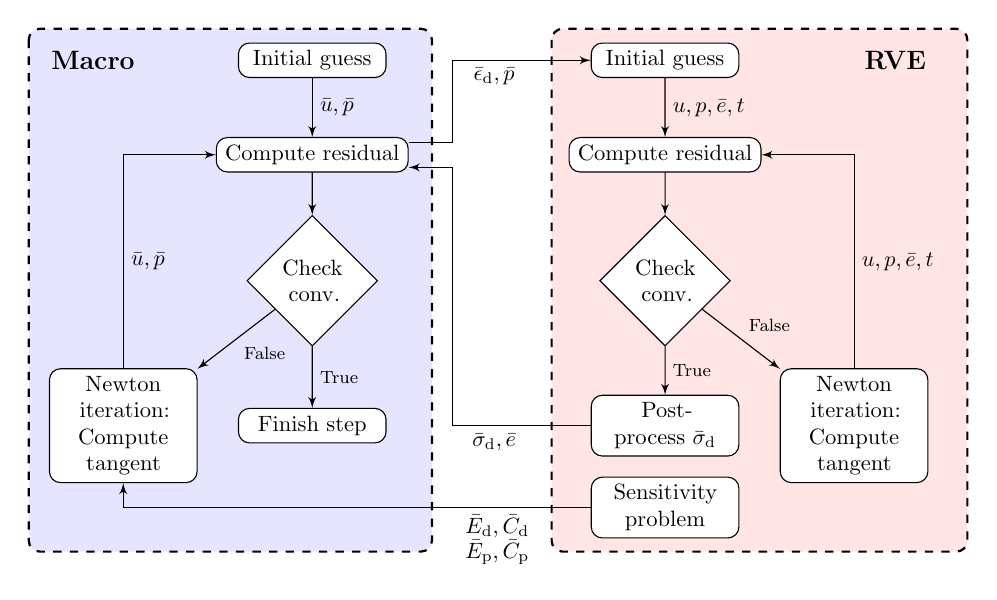
\begin{tikzpicture}[node distance = 2cm, auto,scale=0.8, transform shape]
    %\small
    %\tikzstyle{every node}=[font=\footnotesize]
    \tikzstyle{group}    = [rectangle, draw, thick, dashed, text width=6em, text centered, rounded corners]
    \tikzstyle{decision} = [diamond,   draw, fill=white, text width=4em, text centered, node distance=2.5cm, inner sep=0pt]
    \tikzstyle{block}    = [rectangle, draw, fill=white, text width=6em, text centered, rounded corners]
    \tikzstyle{line}     = [draw, -latex']

    \draw [thick, dashed, fill=blue!10, rounded corners] (-4.5,0.5) rectangle ( 1.9,-7.8);
    \draw [thick, dashed, fill=red!10,  rounded corners] ( 3.8,0.5) rectangle (10.4,-7.8);
    \node [below right, inner sep=10pt] at (-4.5,0.5) { \textbf{\large Macro} };
    \node [below left,  inner sep=10pt] at (10.1,0.5) { \textbf{\large RVE} };

    % Place nodes
    \node [block] (init) {Initial guess};
    \node [block, below of=init, text width=8em, node distance=1.5cm] (residual) {Compute residual};
    \node [decision, below of=residual,node distance=2cm] (convergence) {Check conv.};
    \node [block, below of=convergence, node distance=2.3cm] (stop) {Finish step};
    \node [block, left of=stop, node distance=3cm] (update) {Newton iteration: Compute tangent};
    % Draw edges
    \path [line] (init) -- (residual) node[midway] {$\bar{\ta{u}},\bar{p}$};
    \path [line] (residual) -- (convergence);
    \path [line] (convergence) -- node {\footnotesize False} (update);
    \path [line] (convergence) -- node {\footnotesize True} (stop);
    \path [line] (update) |- node[near start,right] {$\bar{\ta{u}},\bar{p}$} (residual);

    % Place nodes
    \node [block, right of=init, node distance=5.6cm] (rve_init) {Initial guess};
    \node [block, below of=rve_init, text width=8em, node distance=1.5cm] (rve_residual) {Compute residual};
    \node [decision, below of=rve_residual, node distance=2cm] (rve_convergence) {Check conv.};
    \node [block, below of=rve_convergence, node distance=2.3cm] (rve_stop) {Post-process $\bar{\ts\sigma}_\dev$};
    \node [block, right of=rve_stop, node distance=3cm] (rve_update) {Newton iteration: Compute tangent};
    % Sensitivity problem
    \node [block, below of=rve_stop, node distance=1.3cm] (rve_sensitivity) {Sensitivity problem};
    
    % Draw edges
    \path [line] (rve_init) -- (rve_residual) node[midway] {$\ta{u},p,\bar{e},\ta{t}$};
    \path [line] (rve_residual) -- (rve_convergence);
    \path [line] (rve_convergence) -- node {\footnotesize False} (rve_update);
    \path [line] (rve_convergence) -- node {\footnotesize True} (rve_stop);
    \path [line] (rve_update) |- node[right, near start] {$\ta{u},p,\bar{e},\ta{t}$} (rve_residual);

    \path [line] (residual.east) ++(0, 0.2cm) -- ++(0.7cm,0) |- node [below,pos=0.65] {$\bar{\ts \epsilon}_\dev, \bar{p}$} (rve_init);
    % Draw this backwards in order to get exact alignments
    \path [line, latex'-] (residual.east) ++(0,-0.2cm) -- ++(0.7cm,0) |- node [below,pos=0.65] {$\bar{\ts\sigma}_\dev, \bar{e}$} (rve_stop);

    \path [line] (rve_sensitivity) -| node[below, pos=0.10] {$\substack{\displaystyle\bar{\tf E}_\ded,\bar{\ts C}_\ded \\ \displaystyle\bar{\ts E}_\dep,\bar{C}_\dep}$} (update);
\end{tikzpicture}

\end{center}
\end{frame}

%%%%%%%%%%%%%%%%%%%%%%%%%%%%%%%%%%%%%%%%%%%%%%%%%%%%%%%%%%%%%%%%%%%%%%%%%%%%%%%%%%%%%%%%%%%%%%%%%%%
\begin{frame}
 \frametitle{Statistical Volume Element (SVE)}
\begin{center}
 \hspace{1cm}
 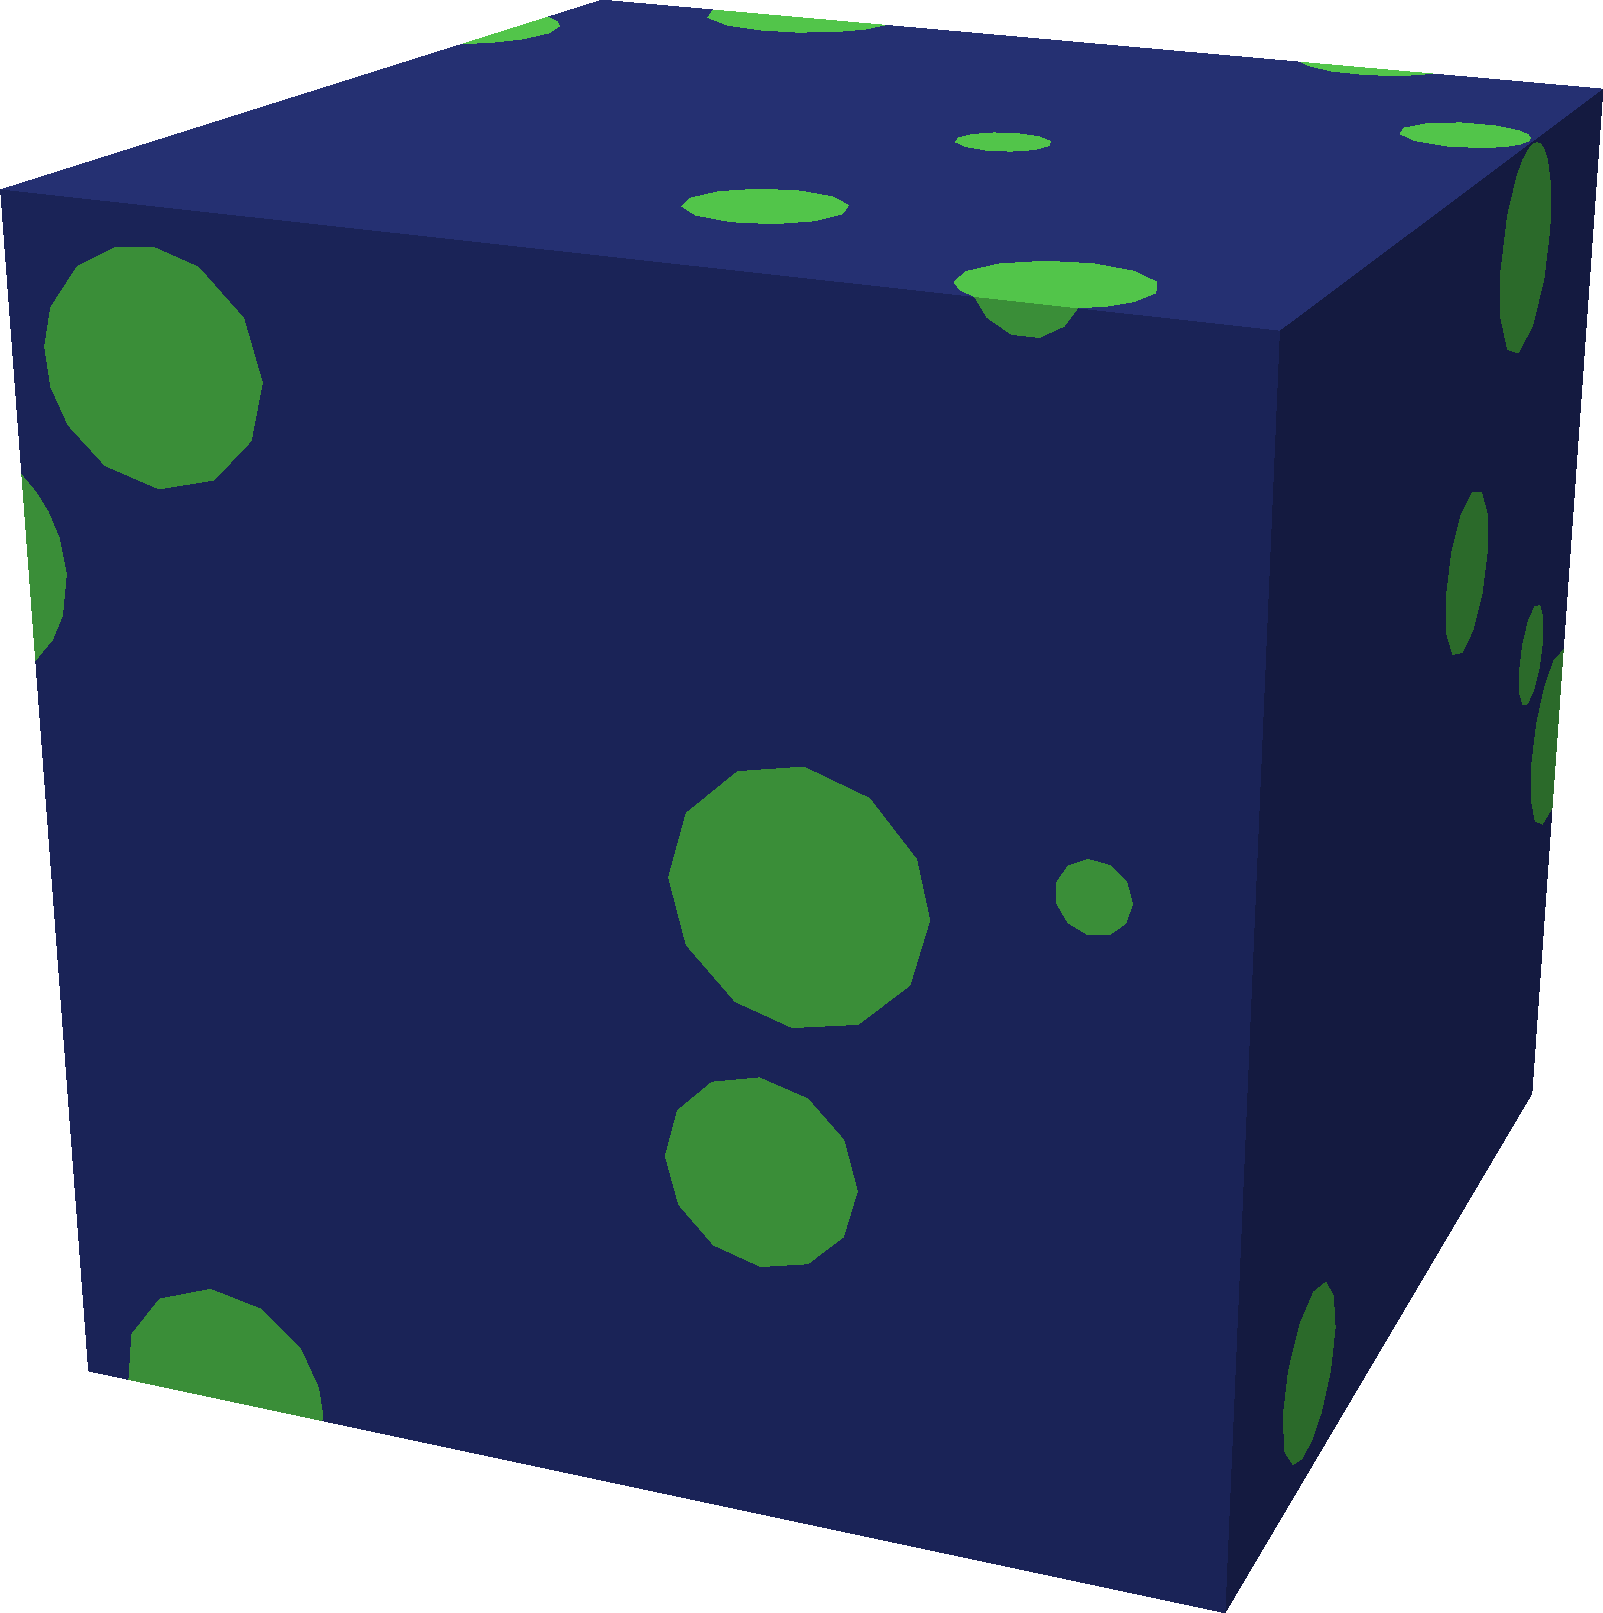
\includegraphics[scale=0.05]{figures/rve6.png}
 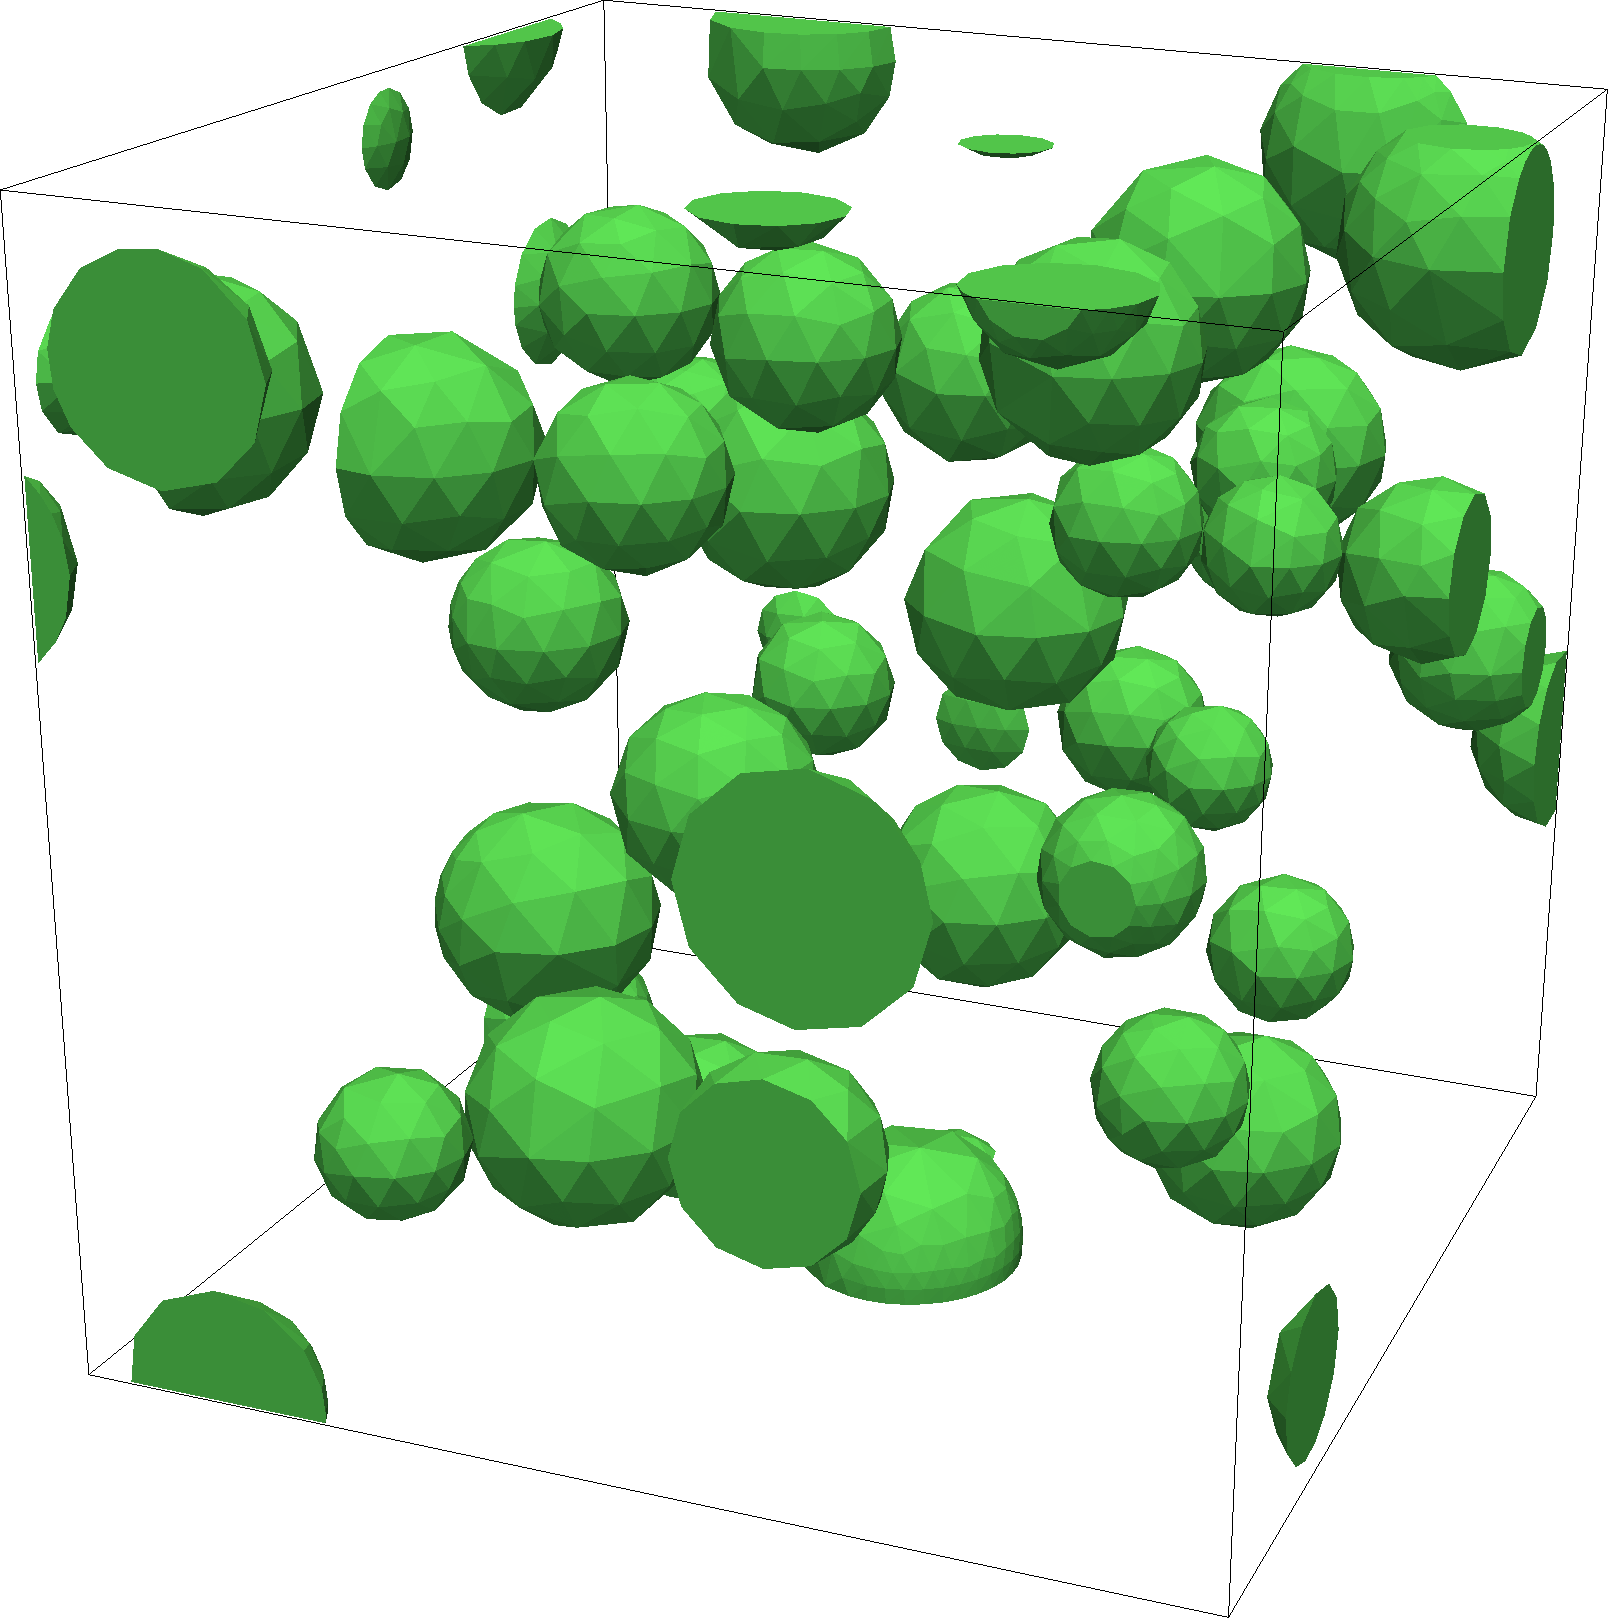
\includegraphics[scale=0.05]{figures/rve6_inc.png}
 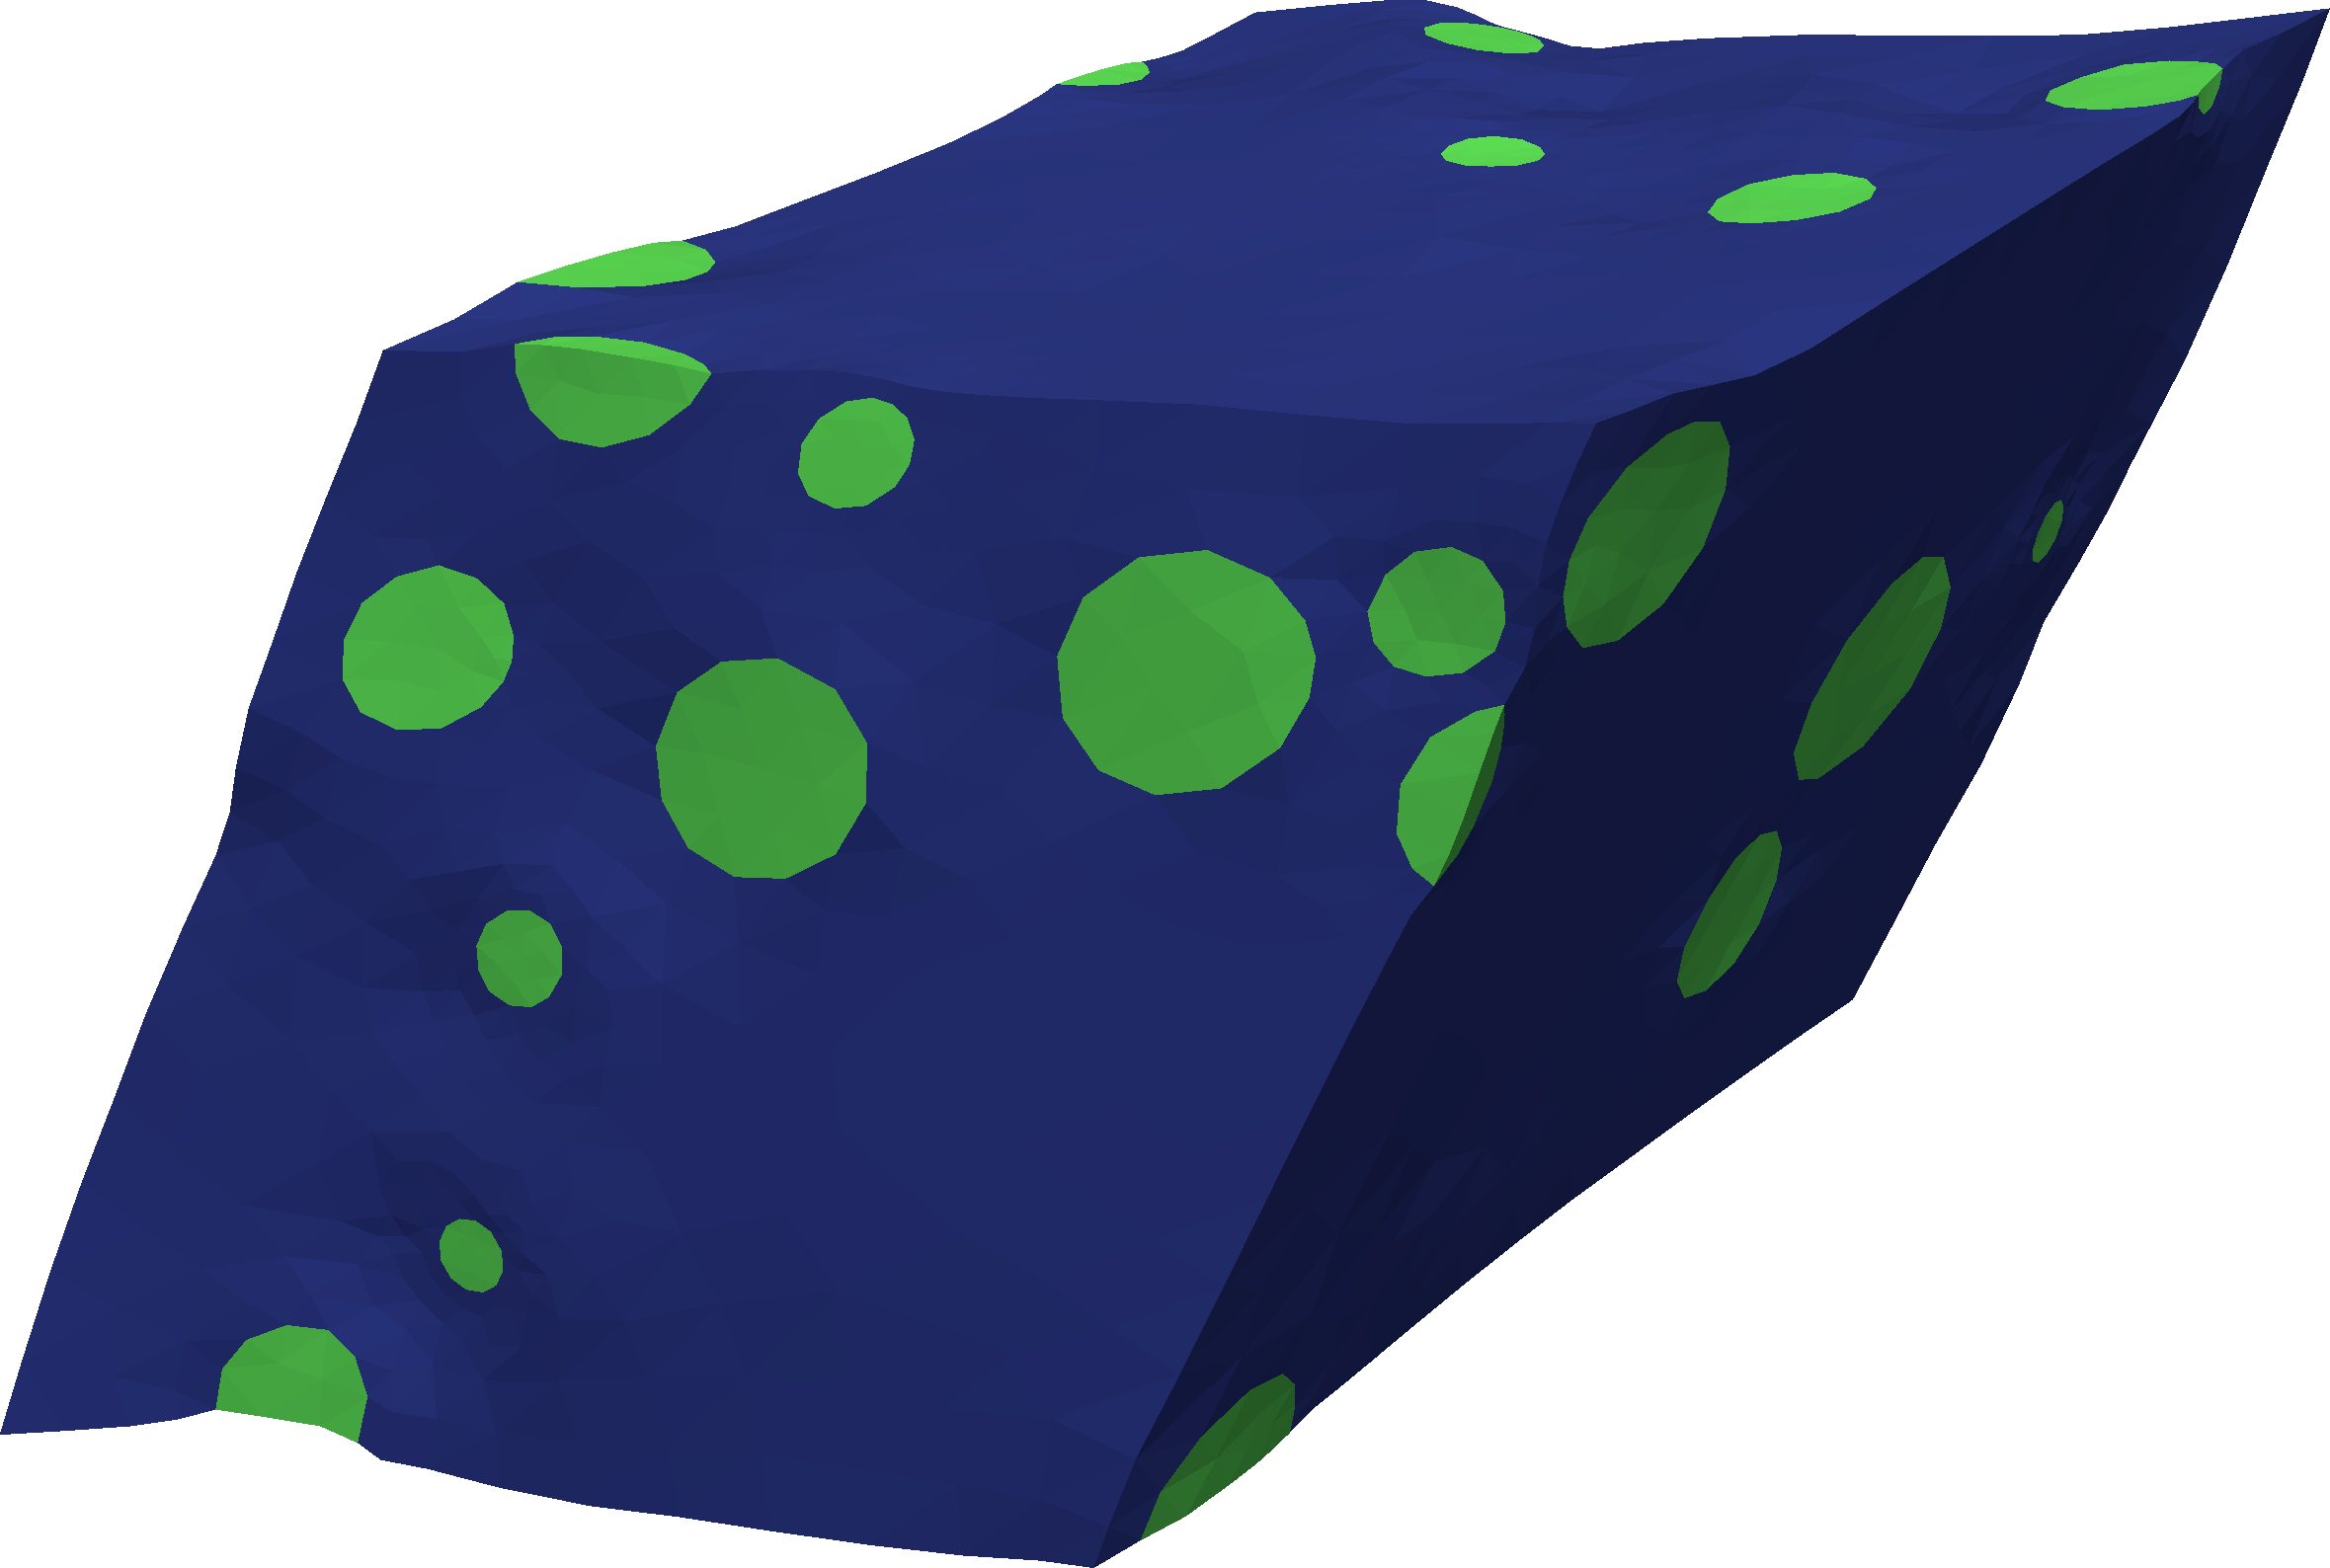
\includegraphics[scale=0.05]{figures/rve6_def.png}
\end{center}
 \begin{align*}
  \hat{\ts\sigma}_\dev(\ts\epsilon_\dev) &= 2 G \ts\epsilon_\dev
\\
  \hat{e}(p) &= -C p = -\frac{1}{K} p
 \end{align*}
\end{frame}

%%%%%%%%%%%%%%%%%%%%%%%%%%%%%%%%%%%%%%%%%%%%%%%%%%%%%%%%%%%%%%%%%%%%%%%%%%%%%%%%%%%%%%%%%%%%%%%%%%%
\begin{frame}
 \frametitle{Homogenized shear and bulk modulus}
\begin{center}
%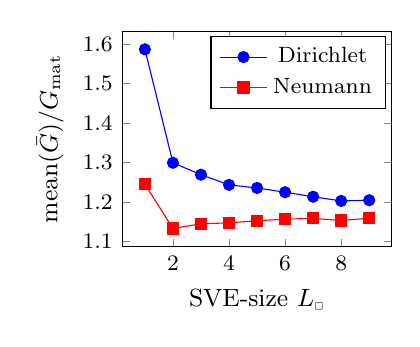
\begin{tikzpicture}
  \begin{axis}[ width=0.5\linewidth, height=0.28\linewidth,
      footnotesize,
      xlabel=SVE-size $L_\rve$, ylabel=$\mathop{\mathrm{mean}}(\bar{G})/G_\mathrm{mat}$]
  \addplot table[color=blue,x=size,y=d_mean] {
size d_mean d_var
1.000000   1.586624   0.489829
2.000000   1.299371   0.029517
3.000000   1.269267   0.007279
4.000000   1.243507   0.002562
5.000000   1.235669   0.000874
6.000000   1.224925   0.000534
7.000000   1.213449   0.000258
8.000000   1.202848   0.000205
9.000000   1.204560   0.000033
  };
 \addlegendentry{Dirichlet}
  \addplot table[color=red,x=size,y=n_mean] {
size n_mean n_var
1.000000   1.245017   0.110729
2.000000   1.133016   0.006438
3.000000   1.144928   0.002252
4.000000   1.147371   0.001132
5.000000   1.152570   0.000572
6.000000   1.156771   0.000293
7.000000   1.158645   0.000139
8.000000   1.153319   0.000129
9.000000   1.158993   0.000039
  };
\addlegendentry{Neumann}
  \end{axis}
\end{tikzpicture}

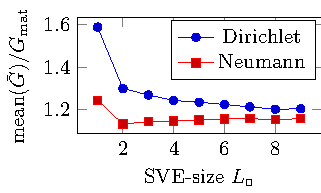
\includegraphics[width=0.4\linewidth]{figures/meanG}
%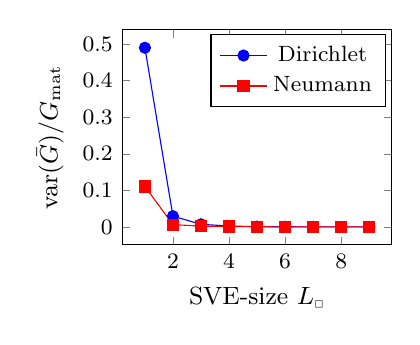
\begin{tikzpicture}
  \begin{axis}[ width=0.50\linewidth, height=0.28\linewidth,
      footnotesize,
      xlabel=SVE-size $L_\rve$, ylabel=$\mathop{\mathrm{var}}(\bar{G})/G_\mathrm{mat}$]
  \addplot table[color=blue,x=size,y=d_var] {
size d_mean d_var
1.000000   1.586624   0.489829
2.000000   1.299371   0.029517
3.000000   1.269267   0.007279
4.000000   1.243507   0.002562
5.000000   1.235669   0.000874
6.000000   1.224925   0.000534
7.000000   1.213449   0.000258
8.000000   1.202848   0.000205
9.000000   1.204560   0.000033
  };
\addlegendentry{Dirichlet}
  \addplot table[color=red,x=size,y=n_var] {
size n_mean n_var
1.000000   1.245017   0.110729
2.000000   1.133016   0.006438
3.000000   1.144928   0.002252
4.000000   1.147371   0.001132
5.000000   1.152570   0.000572
6.000000   1.156771   0.000293
7.000000   1.158645   0.000139
8.000000   1.153319   0.000129
9.000000   1.158993   0.000039
  };
\addlegendentry{Neumann}
  \end{axis}
\end{tikzpicture}

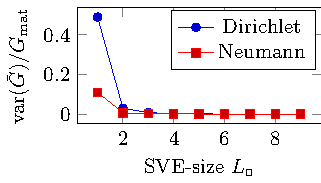
\includegraphics[width=0.4\linewidth]{figures/varG}
\\
$G_\mathrm{part} = 5 G_\mathrm{mat}$, $C_\mathrm{part} = C_\mathrm{mat} = 0$
\\%hline
%\begin{tikzpicture}
  \begin{axis}[ 
    width=0.45\linewidth, height=0.28\linewidth,
    xlabel=$C_\mathrm{mat}\times G_\mathrm{mat}$,
    ylabel=$\bar{C}\times G_\mathrm{mat}$,
    extra x ticks={1.09091, 0.75000, 0.46154, 0.21429, 0.00000},
    extra x tick labels={0.1, 0.2, 0.3, 0.4, 0.5}, 
    every extra x tick/.style = {
        xticklabel style = {name=name label},
        xtick pos = right,
        xticklabel pos = right,
        xtick align = outside
    }
    ]
  \addplot table[color=blue,x=M,y=C] {macro_k9.matdata};
  \end{axis}
  \node at (2.1,2.8) { $\nu_\mathrm{mat}$ };
\end{tikzpicture}

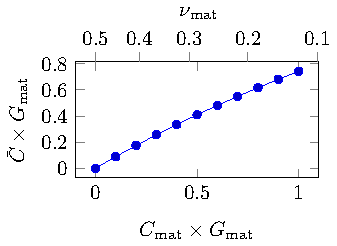
\includegraphics[width=0.4\linewidth]{figures/CGmat}
%\begin{tikzpicture}
  \begin{axis}[
    width=0.45\linewidth, height=0.28\linewidth,
    xlabel=$C_\mathrm{mat}\times G_\mathrm{mat}$,
    ylabel=$\bar{G}/G_\mathrm{mat}$,
    extra x ticks={1.09091, 0.75000, 0.46154, 0.21429, 0.00000},
    extra x tick labels={0.1, 0.2, 0.3, 0.4, 0.5}, 
    every extra x tick/.style = {
        xticklabel style = {name=name label},
        xtick pos = right,
        xticklabel pos = right,
        xtick align = outside
    }
    ]
  \addplot table[color=blue,x=M,y=G] {macro_k9.matdata};
  \end{axis}
  \node at (2.1,2.8) { $\nu_\mathrm{mat}$ };
\end{tikzpicture}

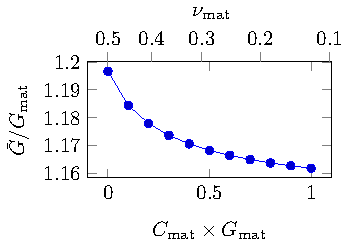
\includegraphics[width=0.4\linewidth]{figures/GGmat}
\\
$G_\mathrm{part} = 5 G_\mathrm{mat}$, $C_\mathrm{part} = 0$
% Homogenized results from a single RVE with Dirichlet boundary condition.
% Dependence of effective properties $\bar{C}$ and $\bar{G}$ on the bulk compliance $C_\mathrm{mat}$ for fixed values of $G_\mathrm{part} = 5\,G_\mathrm{mat}$ and $C_\mathrm{part} = 0$.
\end{center}
\end{frame}

%%%%%%%%%%%%%%%%%%%%%%%%%%%%%%%%%%%%%%%%%%%%%%%%%%%%%%%%%%%%%%%%%%%%%%%%%%%%%%%%%%%%%%%%%%%%%%%%%%%
%%%%%%%%%%%%%%%%%%%%%%%%%%%%%%%%%%%%%%%%%%%%%%%%%%%%%%%%%%%%%%%%%%%%%%%%%%%%%%%%%%%%%%%%%%%%%%%%%%%   D
%%%%%%%%%%%%%%%%%%%%%%%%%%%%%%%%%%%%%%%%%%%%%%%%%%%%%%%%%%%%%%%%%%%%%%%%%%%%%%%%%%%%%%%%%%%%%%%%%%%
\subsection{D}
\begin{frame}
 \frametitle{Paper D}
\begin{center}
 %\fullcite{ohman_new_2014}
Mikael Öhman.
\\[1em]
\textit{A mixed variational format for two-scale analysis of liquid-phase sintering based on variationally consistent homogenization}.
\\[1em]
In preparation
\end{center}
\end{frame}

%%%%%%%%%%%%%%%%%%%%%%%%%%%%%%%%%%%%%%%%%%%%%%%%%%%%%%%%%%%%%%%%%%%%%%%%%%%%%%%%%%%%%%%%%%%%%%%%%%%
\begin{frame}
 \frametitle{Choice of prolongation}
\begin{itemize}
 \item First order Taylor expansion of the velocity, and an (affine and scaled) zeroth order expansion of the pressure 
\begin{align*}
 \ta v^\macro &= \bar{\ta v} + [\bar{\ta v}\outerp\diff]\cdot[\ta x - \bar{\ta x}]
%\label{eq:vm_d}
\\
 p^\macro &= \frac{\volume}{|\Omega_\rve^\particle|}[\bar{p} + \frac23\shomgen{\gamma_\surf}]
%\label{eq:pm_d}
\end{align*}
\item Constraints on the fluctuations $\ta u^\fluct$ and $p^\fluct$ within each RVE via the conditions
\begin{align*}
 \frac{1}{\volume}\int_{\Gamma_\rve}\ta v\outerp\ta n\dif S &= \bar{\ta v}\outerp\diff
%\label{eq:avg_v_d}
\\
 \homgen{p} - \frac23\shomgen{\gamma_\surf} &= \bar{p}
%\label{eq:avg_p_d}
\end{align*}
\end{itemize}
\end{frame}

%%%%%%%%%%%%%%%%%%%%%%%%%%%%%%%%%%%%%%%%%%%%%%%%%%%%%%%%%%%%%%%%%%%%%%%%%%%%%%%%%%%%%%%%%%%%%%%%%%%
\begin{frame}
 \frametitle{Macroscale problem}
\begin{itemize}
 \item Identical macroscale problem to that of Paper B, C
\color{gray}
 \item Find $(\bar{\ta v}, \bar{p}) \in \bar{\set V}\times\bar{\set P}$ such that
 \begin{align*}
  \int_\Omega [{\bar{\ts\sigma}_\dev\{\bar{\ts d}_\dev, \bar{p}\}} - \bar{p}\ts I]\dprod[\delta\bar{\ta v}\outerp\diff]\dif V &= 0\quad \forall \delta\bar{\ta v} \in \bar{\set{V}}^0
\\
  \int_\Omega [-\bar{\ta v}\cdot\diff + {\bar{e}\{\bar{\ts d}_\dev, \bar{p}\}}]\delta\bar{p}\dif V &= 0\quad \forall \delta\bar{p} \in \bar{\set{P}}
 \end{align*}
 \item RVE-input: $\bar{\ts d}_\dev\defeq [\bar{\ta v}\outerp\diff]^\sym_\dev$ and $\bar{p}$.
 \item The homogenized response variables are identified as
 \begin{align*}
 \bar{\ts\sigma}_\dev &\defeq \frac{1}{\volume} \left[\int_{\Gamma_\rve} \ta t \outerp [\ta x-\bar{\ta x}]\dif S\right]_\dev
\\
 \bar{e} &\defeq \frac{1}{\volume} \int_{\Gamma_\rve} \ta v \cdot \ta n\dif S
 \end{align*}
\color{black}
 \item \textbf{Remark}: No pores intersecting the RVE-boundary allowed!
\end{itemize}
\end{frame}

% %%%%%%%%%%%%%%%%%%%%%%%%%%%%%%%%%%%%%%%%%%%%%%%%%%%%%%%%%%%%%%%%%%%%%%%%%%%%%%%%%%%%%%%%%%%%%%%%%%%
% \begin{frame}
%  \frametitle{Comments}
% \begin{itemize}
%  \item The Dirichlet boundary condition is identical to that in Paper B.
% \end{itemize}
% \end{frame}

%%%%%%%%%%%%%%%%%%%%%%%%%%%%%%%%%%%%%%%%%%%%%%%%%%%%%%%%%%%%%%%%%%%%%%%%%%%%%%%%%%%%%%%%%%%%%%%%%%%
\begin{frame}
 \frametitle{RVE problem --- Weakly Periodic b.c.}
\begin{itemize}
 \item For given macroscale variables $\bar{\ts d}_\dev$ and $\bar{p}$, find ($\ta{v},p,\ta t, \bar{e})\in\set{V}_\rve\times\set{P}_\rve\times\set{T}_\rve\times\set R$ that solve the system
%----------------------------------------------------------------------------
\begin{flalign*}
  \downlight{\int_{\mathrlap{\Omega_\rve^\particle}} [\hat{\ts\sigma}_\dev([\ta v \outerp\diff]^\sym_\dev)-p\ts I]\dprod[\delta\ta v \outerp\diff] \dif V }
    - \int_{\mathrlap{\Gamma_\rve^+}} \ta t\cdot\jump{\delta\ta v}\dif S &\downlight{= \int_{\mathrlap{\Gamma_\rve^\pore}} \gamma_\surf[\delta\ta v\cdot\hat{\diff}]\dif S}
\end{flalign*}
\vspace{-2em}
\begin{flalign*}
&&
  \downlight{\forall\;\delta\ta v \in \set V_\rve}
\\
  \downlight{\int_{\mathrlap{\Omega_\rve^\particle}} -\delta p[\ta v \cdot\diff - \hat{e}(p)] \dif V }&\downlight{= 0}
&
  \downlight{\forall\;\delta p \in \set P_\rve}
\\
  -\int_{\mathrlap{\Gamma_\rve^+}} \delta\ta t\cdot \jump{\ta v - \bar{e}\frac13\ta x} \dif S &= -\int_{\mathrlap{\Gamma_\rve^+}} \delta\ta t\cdot \jump{\highlight{\bar{\ts d}_\dev}\cdot\ta x} \dif S
&
  \forall\;\delta\ta t \in \set T_\rve
\\
  \int_{\mathrlap{\Gamma_\rve^+}} \ta t \cdot \jump{\frac13\ta x} \dif S \,\delta\bar{e} &= - \highlight{\bar{p}} \,\delta\bar{e}
&
  \forall\;\delta\bar{e} \in \set R
\end{flalign*}
\end{itemize}
\end{frame}

%%%%%%%%%%%%%%%%%%%%%%%%%%%%%%%%%%%%%%%%%%%%%%%%%%%%%%%%%%%%%%%%%%%%%%%%%%%%%%%%%%%%%%%%%%%%%%%%%%%
% \begin{frame}
%  \frametitle{RVE problem}
% \begin{itemize}
%  \item Weakly Periodic boundary condition
%   \begin{itemize}
%    \item Unknowns: $\ta v$, $p$, $\ta t$, $\bar{e}$.
%    \item Traction $\ta t$ serves as Lagrange multipliers on $\Gamma_\rve$.
%    \item Volumetric deformation $\bar{e}$ serves as a Lagrange multiplier for the mean part of $\ta t$ (simplifies the function space for $\ta t$).
%   \end{itemize}
%  \item Neumann boundary condition 
%   \begin{itemize}
%    \item Unknowns: $\ta v$, $p$, $\bar{\ts\sigma}_\dev$.
%    \item Stress $\bar{\ts\sigma}_\dev$ on $\Gamma_\rve$ serves as a Lagrange multiplier.
%   \end{itemize}
%  \item Dirichlet boundary condition 
%   \begin{itemize}
%    \item Unknowns $\ta v$, $p$, $\bar{e}$.
%   \end{itemize}
%  \item Neumann and Dirichlet conditions provide energy bounds for the Weakly Periodic boundary condition.
% \end{itemize}
% \end{frame}

%%%%%%%%%%%%%%%%%%%%%%%%%%%%%%%%%%%%%%%%%%%%%%%%%%%%%%%%%%%%%%%%%%%%%%%%%%%%%%%%%%%%%%%%%%%%%%%%%%%
\begin{frame}
 \frametitle{Paper D summarized}
\begin{center}
 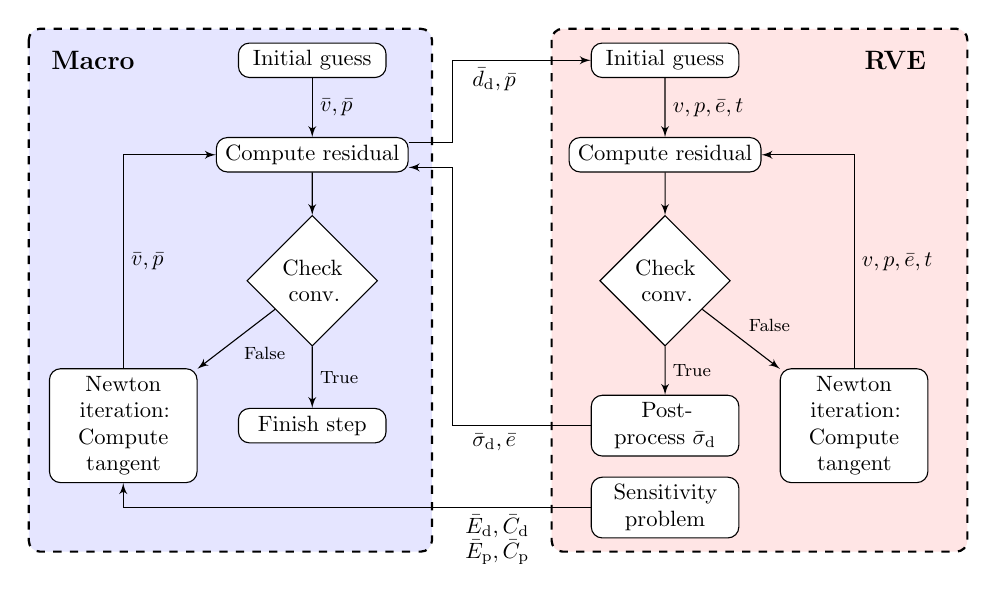
\begin{tikzpicture}[node distance = 2cm, auto,scale=0.8, transform shape]
    %\small
    %\tikzstyle{every node}=[font=\footnotesize]
    \tikzstyle{group}    = [rectangle, draw, thick, dashed, text width=6em, text centered, rounded corners]
    \tikzstyle{decision} = [diamond,   draw, fill=white, text width=4em, text centered, node distance=2.5cm, inner sep=0pt]
    \tikzstyle{block}    = [rectangle, draw, fill=white, text width=6em, text centered, rounded corners]
    \tikzstyle{line}     = [draw, -latex']

    \draw [thick, dashed, fill=blue!10, rounded corners] (-4.5,0.5) rectangle ( 1.9,-7.8);
    \draw [thick, dashed, fill=red!10,  rounded corners] ( 3.8,0.5) rectangle (10.4,-7.8);
    \node [below right, inner sep=10pt] at (-4.5,0.5) { \textbf{\large Macro} };
    \node [below left,  inner sep=10pt] at (10.1,0.5) { \textbf{\large RVE} };

    % Place nodes
    \node [block] (init) {Initial guess};
    \node [block, below of=init, text width=8em, node distance=1.5cm] (residual) {Compute residual};
    \node [decision, below of=residual,node distance=2cm] (convergence) {Check conv.};
    \node [block, below of=convergence, node distance=2.3cm] (stop) {Finish step};
    \node [block, left of=stop, node distance=3cm] (update) {Newton iteration: Compute tangent};
    % Draw edges
    \path [line] (init) -- (residual) node[midway] {$\bar{\ta{v}},\bar{p}$};
    \path [line] (residual) -- (convergence);
    \path [line] (convergence) -- node {\footnotesize False} (update);
    \path [line] (convergence) -- node {\footnotesize True} (stop);
    \path [line] (update) |- node[near start,right] {$\bar{\ta{v}},\bar{p}$} (residual);

    % Place nodes
    \node [block, right of=init, node distance=5.6cm] (rve_init) {Initial guess};
    \node [block, below of=rve_init, text width=8em, node distance=1.5cm] (rve_residual) {Compute residual};
    \node [decision, below of=rve_residual, node distance=2cm] (rve_convergence) {Check conv.};
    \node [block, below of=rve_convergence, node distance=2.3cm] (rve_stop) {Post-process $\bar{\ts\sigma}_\dev$};
    \node [block, right of=rve_stop, node distance=3cm] (rve_update) {Newton iteration: Compute tangent};
    % Sensitivity problem
    \node [block, below of=rve_stop, node distance=1.3cm] (rve_sensitivity) {Sensitivity problem};
    
    % Draw edges
    \path [line] (rve_init) -- (rve_residual) node[midway] {$\ta{v},p,\bar{e},\ta{t}$};
    \path [line] (rve_residual) -- (rve_convergence);
    \path [line] (rve_convergence) -- node {\footnotesize False} (rve_update);
    \path [line] (rve_convergence) -- node {\footnotesize True} (rve_stop);
    \path [line] (rve_update) |- node[right, near start] {$\ta{v},p,\bar{e},\ta{t}$} (rve_residual);

    \path [line] (residual.east) ++(0, 0.2cm) -- ++(0.7cm,0) |- node [below,pos=0.65] {$\bar{\ts d}_\dev, \bar{p}$} (rve_init);
    % Draw this backwards in order to get exact alignments
    \path [line, latex'-] (residual.east) ++(0,-0.2cm) -- ++(0.7cm,0) |- node [below,pos=0.65] {$\bar{\ts\sigma}_\dev, \bar{e}$} (rve_stop);

    \path [line] (rve_sensitivity) -| node[below, pos=0.10] {$\substack{\displaystyle\bar{\tf E}_\ded,\bar{\ts C}_\ded \\ \displaystyle\bar{\ts E}_\dep,\bar{C}_\dep}$} (update);
\end{tikzpicture}

\end{center}
\end{frame}

%%%%%%%%%%%%%%%%%%%%%%%%%%%%%%%%%%%%%%%%%%%%%%%%%%%%%%%%%%%%%%%%%%%%%%%%%%%%%%%%%%%%%%%%%%%%%%%%%%%
\begin{frame}
 \frametitle{Numerical results for 2D RVE: Free sintering $\bar{p} = 0$}
\begin{center}
 \begin{tikzpicture}
  \node at (0,0) {
\includegraphics[scale=0.15]{figures/initial_rve}};
  \node at (4,2) {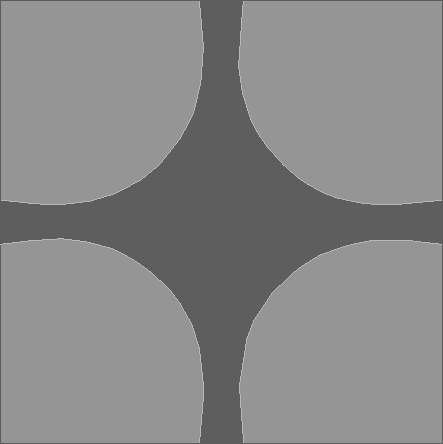
\includegraphics[scale=0.15]{figures/final_dirichlet}};
  \node at (4,-2) {
\includegraphics[scale=0.15]{figures/final_neumann}};
  \node at (0,1.5) {Initial};
  \node at (4,3.5) {Dirichlet};
  \node at (4,-0.5) {Neumann};
  \draw[-latex] (1.5,0.5) -- (2.5,1);
  \draw[-latex] (1.5,-0.5) -- (2.5,-1);
  \node at (8,2) {
\includegraphics[scale=0.2]{figures/rve_dirichlet_2}};
  \node at (8,-2) {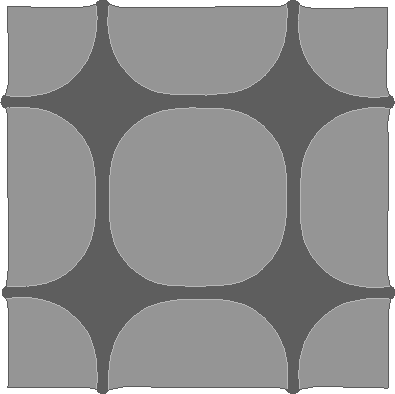
\includegraphics[scale=0.2]{figures/rve_neumann_2}};
 \end{tikzpicture}
\end{center}
\end{frame}

%%%%%%%%%%%%%%%%%%%%%%%%%%%%%%%%%%%%%%%%%%%%%%%%%%%%%%%%%%%%%%%%%%%%%%%%%%%%%%%%%%%%%%%%%%%%%%%%%%%
\begin{frame}
 \frametitle{Numerical results for 2D RVE: Free sintering $\bar{p} = 0$}
\begin{center}
\begin{tikzpicture}
 \begin{axis}[
    width=1.0\linewidth,
    height=0.5\linewidth,
    ylabel={Relative density},xlabel={Time (scaled by end time)},
    xmax=1, xmin=0, ymax=1.01, ymin=0.83,
    cycle list name=linestyles,
    yticklabel style={font=\tiny}, xticklabel style={font=\tiny},
%     scaled y ticks=manual:{}{\pgfmathparse{#1*100}}, % Scale for percentage
%     scaled x ticks=manual:{}{\pgfmathparse{#1*1000}}, % Scale for percentage
    legend style={draw=black,rounded corners=3pt,font=\tiny},
    legend pos=south east
    ]
  \addplot[blue ,densely dashed] table[y index=2] {figures/macro_3_dirichlet_x.out.matdata};
  \addlegendentry {Dirichlet 3$\times$3}
  \addplot[red  ,densely dashed] table[y index=2] {figures/macro_2_dirichlet_x.out.matdata};
  \addlegendentry {Dirichlet 2$\times$2}
  \addplot[black,densely dashed] table[y index=2] {figures/macro_1_dirichlet_x.out.matdata};
  \addlegendentry {Dirichlet 1$\times$1}

  \addplot[blue ] table[y index=2] {figures/macro_3_neumann_x.out.matdata};
  \addlegendentry {Neumann 3$\times$3}
  \addplot[red  ] table[y index=2] {figures/macro_2_neumann_x.out.matdata};
  \addlegendentry {Neumann 2$\times$2}
  \addplot[black] table[y index=2] {figures/macro_1_neumann_x.out.matdata};
  \addlegendentry {Neumann 1$\times$1}
 \end{axis}
\end{tikzpicture}
\end{center}
\end{frame}

%%%%%%%%%%%%%%%%%%%%%%%%%%%%%%%%%%%%%%%%%%%%%%%%%%%%%%%%%%%%%%%%%%%%%%%%%%%%%%%%%%%%%%%%%%%%%%%%%%%
\begin{frame}
 \frametitle{Numerical results for 3D RVE: Macroscale shear}
\begin{center}
 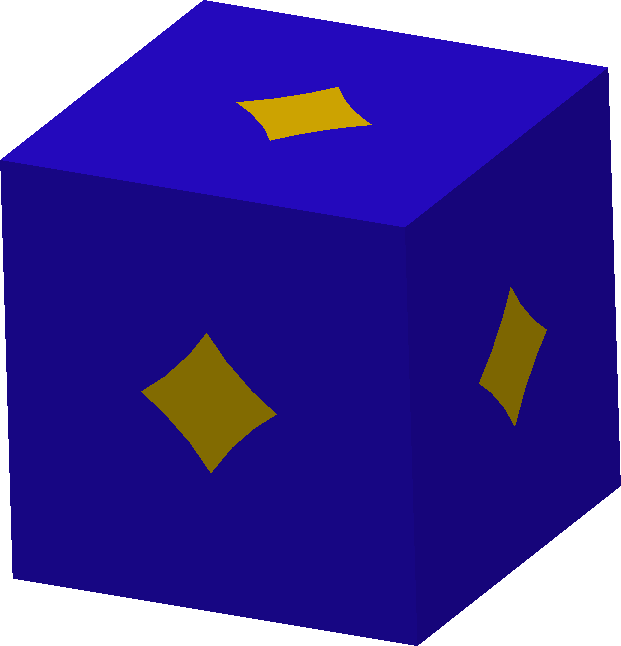
\includegraphics[height=0.3\linewidth]{figures/eightspheres}
 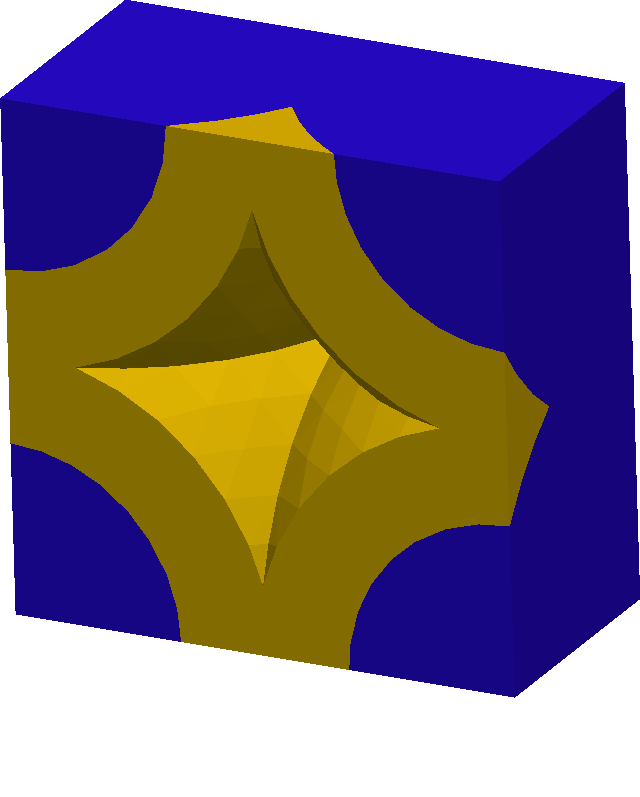
\includegraphics[height=0.3\linewidth]{figures/eightspheres_cut}
\\
 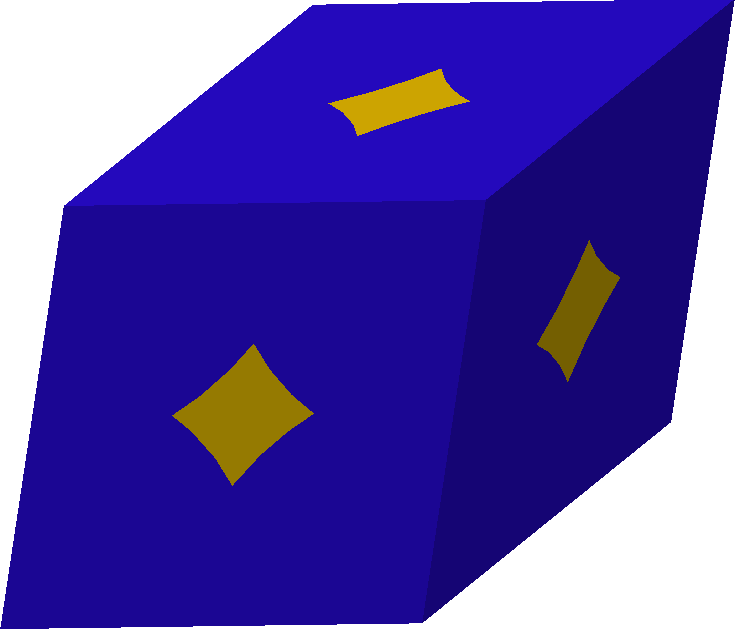
\includegraphics[width=0.3\linewidth]{figures/eightspheres_d_shear}
 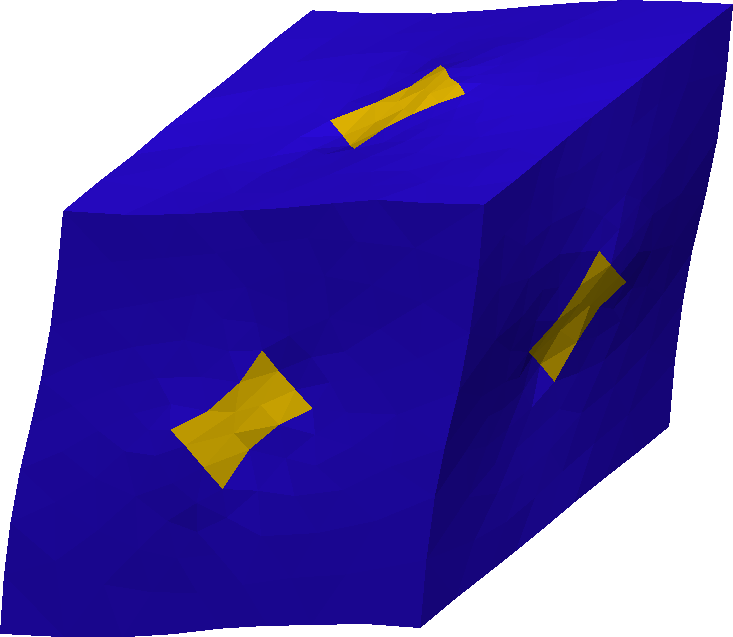
\includegraphics[width=0.3\linewidth]{figures/eightspheres_p_shear}
 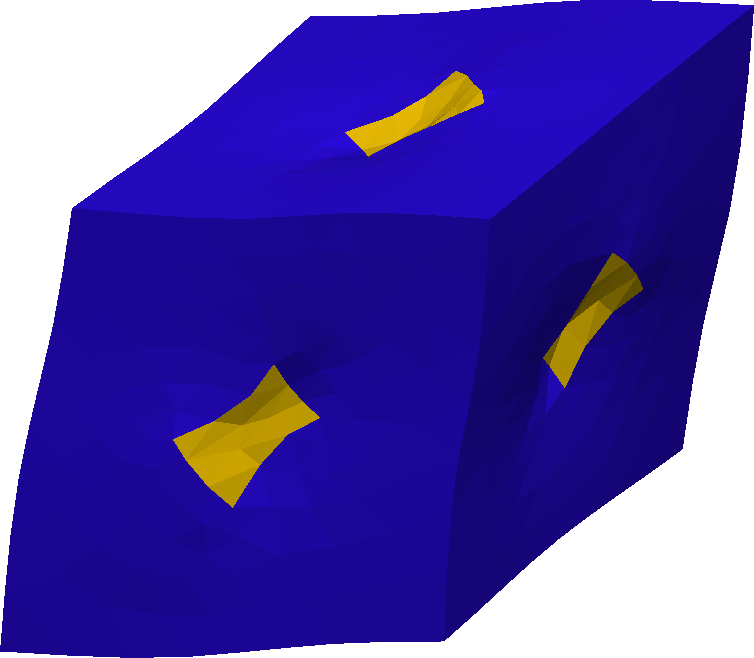
\includegraphics[width=0.3\linewidth]{figures/eightspheres_n_shear}
 %\caption{3D unit-cell subject to pure shear. Boundary conditions are in order; Dirichlet, weakly periodic, and Neumann}
\end{center}
\end{frame}

%%%%%%%%%%%%%%%%%%%%%%%%%%%%%%%%%%%%%%%%%%%%%%%%%%%%%%%%%%%%%%%%%%%%%%%%%%%%%%%%%%%%%%%%%%%%%%%%%%%
\begin{frame}
 \frametitle{Numerical results for 3D RVE: No macroscale deformation}
\begin{center}
 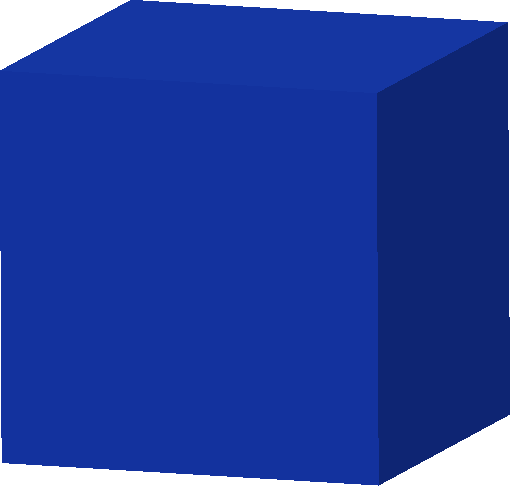
\includegraphics[height=0.3\linewidth]{figures/RVEAniso}
\hspace{1cm}
 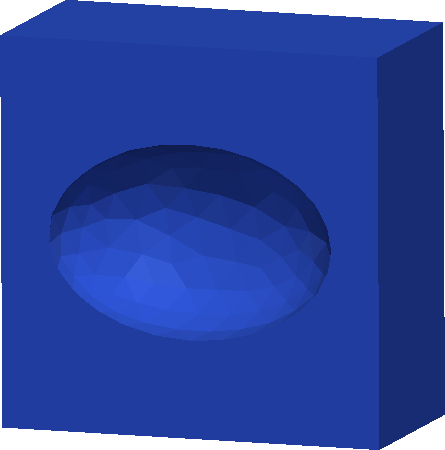
\includegraphics[height=0.3\linewidth]{figures/RVEAnisoCut}
 %\caption{3D unit-cell subject to pure shear. Boundary conditions are in order; Dirichlet, weakly periodic, and Neumann}
\end{center}
 \begin{itemize}
  \item No macroscale deformation $\leadsto$ ``sintering stress'' is obtained:
  \begin{align*}
   \bar{e} = 0 &\rightarrow \bar{p} = -6.96 \frac{\gamma_\surf}{L}
\\
   \bar{\ts d}_\dev = \ts 0 &\rightarrow \bar{\ts\sigma}_\dev = \left[\begin{smallmatrix} 0.149 & 0 & 0 \\ 0 & -0.075 & 0 \\ 0 & 0 & -0.074 \end{smallmatrix}\right]\frac{\gamma_\surf}{L}
  \end{align*}
 \item \textbf{Remark} Anisotropy due to topology
 \end{itemize}
\end{frame}




%%%%%%%%%%%%%%%%%%%%%%%%%%%%%%%%%%%%%%%%%%%%%%%%%%%%%%%%%%%%%%%%%%%%%%%%%%%%%%%%%%%%%%%%%%%%%%%%%%%
\begin{frame}
 \frametitle{Conclusions}
 \begin{itemize}
 \item Variationally consistent homogenization suitable for sintering. Modeling framework allows for
  \begin{enumerate}
   \item surface tension
   \item seamless transition to macroscopic incompressibility (for vanishing porosity)
  \end{enumerate}
 %\item Homogenization for mixed $(\ta u, p)$-formulated elasticity
 \item FE\textsuperscript{2} implementation $\leadsto$ Prediction of final shape, i.e.\ a simulation tool towards the design of near.net-shape manufacturing
 \item Evolving mesoscale topology: Surface tracking and remeshing algorithm
 \item Numerical results for Weakly Periodic, Dirichlet, and Neumann boundary conditions on RVE
  \begin{enumerate}
   \item ``Sintering stress'' is highly dependent on pore shape (possibly anisotropic), advantage over macroscopic models!
   \item Bulk modulus of constituents can affect effective macroscopic shear modulus
   \item ``Hard'' particles $\leadsto$ Neumann boundary condition becomes an efficient alternative to periodicity
  \end{enumerate}
 \end{itemize}
% In this thesis a novel approach to simulate the sintering process as a problem of computational homogenization is presented, replacing traditional (macroscopic) constitutive modeling.
% With the proposed homogenization procedure, a seamless transition from the macroscopically compressible to the incompressible response is ensured, which is of vital importance when modeling sintering of particle composites.
% 
% Through rigorously applying VCH, we can ensure that the obtained macroscale problem is sound, and the RVE-problem retains the same strong form as the fine scale problem.
% These properties allow for a straightforward FE-implementation.
% 
% For the homogenization procedure, pores on the RVE-boundaries remain complicated.
% Weakly periodic and Neumann boundary conditions are not applicable, while Dirichlet boundary conditions constrains the closing of pores on the boundary.
% A strongly periodic boundary condition could therefore be a necessity for RVEs with pores intersecting the boundary, but makes it considerably harder to (re)generate a mesh.
\end{frame}

%%%%%%%%%%%%%%%%%%%%%%%%%%%%%%%%%%%%%%%%%%%%%%%%%%%%%%%%%%%%%%%%%%%%%%%%%%%%%%%%%%%%%%%%%%%%%%%%%%%
\begin{frame}
 \frametitle{Future work}
 \begin{itemize}
  \item Alternatives to traditional meshing (e.g.\ Particle FEM, Level-sets)
  \item Improved subscale modeling
   \begin{itemize}
    \item Material models for WC and Co (elasto-viscoplastic, temperature dependence)
    \item Microstructure topology
    \item Surface diffusion
   \end{itemize}
  \item Improved RVE-problem formulation: Boundary conditions to deal with pores intersecting the boundary
%   \item Pores intersecting with boundaries are problematic. Possible solutions are
%    \begin{itemize}
%     \item strongly periodic boundary condition
%     \item modified Neumann boundary condition
%    \end{itemize}
 \end{itemize}
\end{frame}



% 
% 
% %%%%%%%%%%%%%%%%%%%%%%%%%%%%%%%%%%%%%%%%%%%%%%%%%%%%%%%%%%%%%%%%%%%%%%%%%%%%%%%%%%%%%%%%%%%%%%%%%%%
% \begin{frame}
% \frametitle{The final pieces}
%  \begin{itemize}
%   \item Large toplogical changes requires remeshing
%   \begin{itemize}
%   \item Added Triangle bindings (\roughcite{J. Schewchuck})
%   \item Topology-tracker: Points tracking surface geometry
%   \item Mesh quality ``error''-estimator to determine when to re-mesh.
%   \end{itemize}
%  \item Surface tension loading implemented as an active boundary condition (should work automatically for all standard elements).
%  \end{itemize}
% \end{frame}

\end{document}
